\section{Simulação}

A simulação do sistema composto por elementos não lineares operando juntamente com filtros ativos conectados na rede de um sistema elétrico aeronáutico é apresentada a seguir. A proposta dessa simulação é criar em ambiente Simulink um sistema típico de geração e distribuição elétrica de uma aeronave de maneira suficientemente completa para analisar os aspectos operacionais de filtros ativos, além de observar suas características operando com elementos reais em uma rede elétrica aeronáutica. O foco desse estudo não recai no detalhamento do sistema ao ponto de modelar sistemas de proteção e integração, sendo que isso pode ser trabalho para estudos posteriores.

As características do sistema modelado são realizadas tomando como base uma aeronave de transporte civil com capacidade de uma média de 100 passageiros, tal como uma aeronave EMB-190. Em tais aeronaves o sistema de geração é composto por mais de um gerador, entretanto, em operação normal, os canais de geração são segregados, sendo que será simulado apenas um canal de geração e distribuição. Visto que o foco nesse trabalho não contempla integração de vários sistemas alimentados eletricamente, a carga será toda composta por elementos iguais e não lineares, sendo que estes devem ser propícios a operar com filtros ativos. Dessa maneira, foi determinada a carga sendo constituída por três EHAs operando simultaneamente, sob o mesmo regime de carregamento e sendo atuado no mesmo instante. Esta condição pode ser realizada em uma aeronave com a atuação de alguns EHAs em uma mesma superfície de controle.

\subsection{Modelo do Sistema Elétrico}

\subsubsection{Sistema de Geração}

O sistema de geração aplicado na simulação visa representar de maneira suficientemente apropriada uma fonte de tensão comumente encontrada em sistemas elétricos aeronáuticos. A potência do gerador especificada para o sistema elétrico em um canal de geração é definido como 50 kVA, sendo este valor compatível com o porte da aeronave sob estudo. O bloco de geração montado no Simulink é composto por uma máquina síncrona, cuja entrada mecânica é definida por um valor constante representado pela rotação do eixo proveniente do IDG, e os níveis de tensão é determinado por controle de campo de excitação. Esse último é obtido por uma GCU, a qual opera juntamente com a maquina síncrona do gerador. Em sistemas elétricos aeronáuticos reais a complexidade do bloco Gerador/GCU é elevada e envolve sistemas complementares para garantir sua confiabilidade. Entretanto, para a proposta de simulação apresentado nesse trabalho o sistema proposto por \cite{Olivier} mostra-se adequado. Isto se deve principalmente pela característica da saída do gerador apresentar tensão com frequência definida, com amplitude controlada e pela inclusão das não idealidades representadas pelas resistências e indutâncias nas linhas do gerador.

Em ambiente Simulink tanto o bloco da máquina síncrona como o bloco de excitação de campo estão presentes. Sendo assim o sistema de geração utilizado no software é mostrado na Figura \ref{fig:GEN_GCU.png}.

\begin{figure}[!htb] %
	\centering
	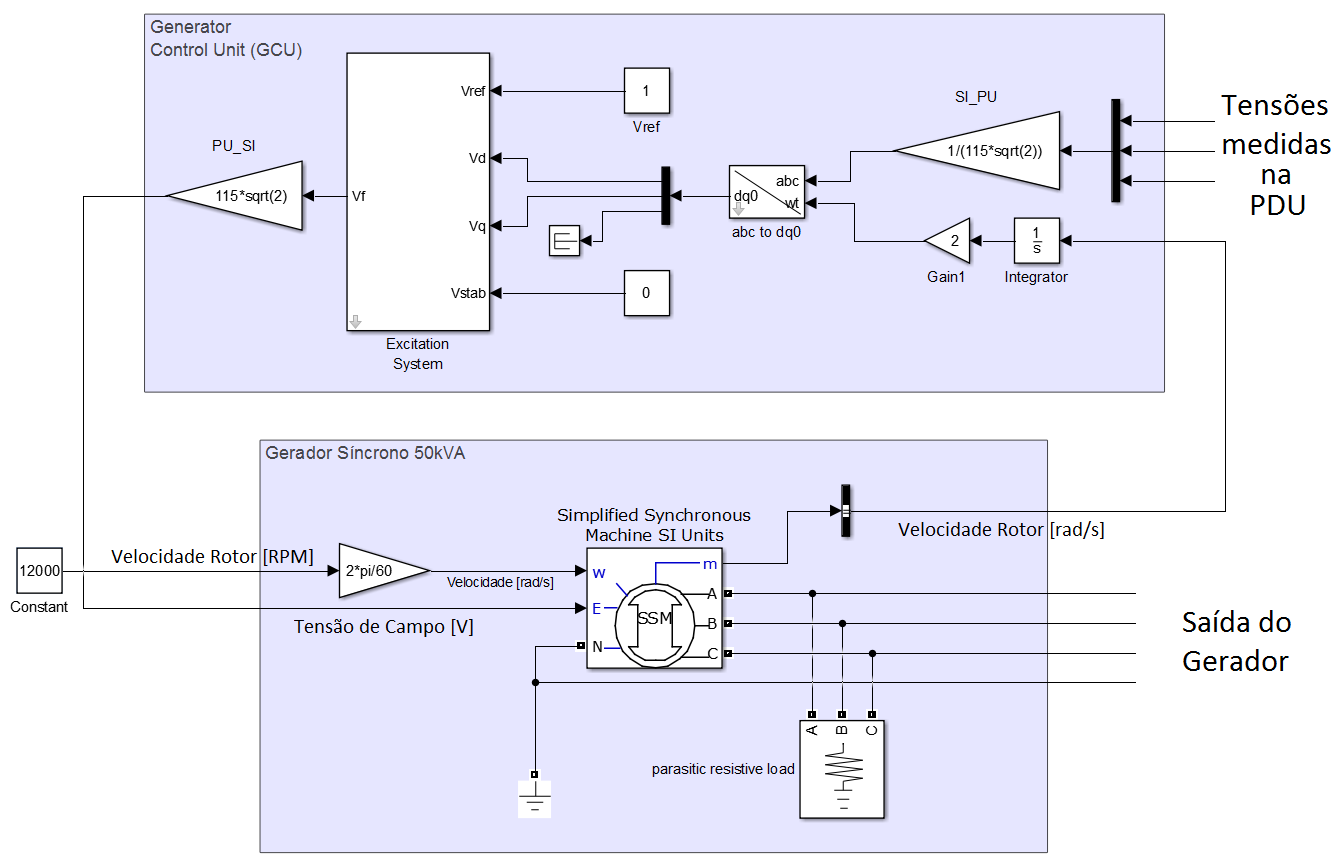
\includegraphics[width=0.99\textwidth]{Cap4/Figuras/GEN_GCU.png}
	\caption{Modelo do sistema de geração}
	\label{fig:GEN_GCU.png}
\end{figure}

Nessa ilustração o subconjunto superior é composto pelos elementos que modelam a GCU. O \textit{Excitation System} é um bloco nativo do Simulink e opera como descrito em \cite{IEEE}. Já os blocos auxiliares da GCU estão presentes para condicionar o sinal adequadamente à operação do \textit{Excitation System}. A medição de tensão que alimenta a GCU deve ser proveniente do barramento de distribuição, visto que as impedâncias da máquina elétrica e sistema de distribuição alterem os níveis de tensão desse ponto em comparação à saída do gerador.

O subconjunto inferior compõe o gerador. A máquina síncrona é também um bloco presente no Simulink e em sua saída estão presentes as resistências e indutâncias conectadas em série, cujos valores são expostos na Tabela \ref{tab:Zgen}.  Ainda existe uma resistência parasita no sistema com o intuito de evitar problemas numéricos na simulação. A presença deste elemento não influencia o sistema que será simulado.

\begin{table}[!htb]
	\centering
	\begin{tabular}{|c|c|c|}
		\hline
		\textbf{Resistência	[$\Omega$]}	& \textbf{Indutância [mH]}	& \textbf{Impedância (400 Hz) [$\Omega$]}\\\hline
		0.0404					& 0.09204			& $0.0404+j0.213$\\
		\hline
	\end{tabular}
	\caption{Impedância interna do Gerador}
	\label{tab:Zgen}
\end{table}

\subsubsection{Sistema de Distribuição}

O sistema de distribuição de uma aeronave é constituído pelos condutores que transferem a energia entre os subsistemas, além dos barramentos de distribuição e equipamentos de proteção do sistema elétrico. Contudo, nesse trabalho as proteções não estão no escopo da simulação, sendo que o modelo proposto será composto apenas pelas linhas de transmissão e um barramento a qual as cargas possam ser conectadas.

O ponto de conexão em comum está localizado na PDU (\textit{Primary Distribution Unit}). Apenas um barramento será considerado e as cargas não lineares compostas pelos EHAs serão conectadas em paralelo a partir dessa unidade. A Figura \ref{fig:dist.png} apresenta o modelo implementado no Simulink para realização da simulação. Aqui pode-se observar as cargas compostas pelos EHAs sendo conectadas a partir da PDU. A alimentação da PDU é realizada diretamente pelo gerador através de uma linha de transmissão trifásica. Nessa unidade ainda existe um sensor de tensão que cede informação ao GCU para o controle de excitação de campo, a qual fornecer ao gerador o controle para que este apresente níveis de tensão adequados para manter a tensão de fase no PCC sendo 115 V.

\begin{figure}[!htb] %
	\centering
	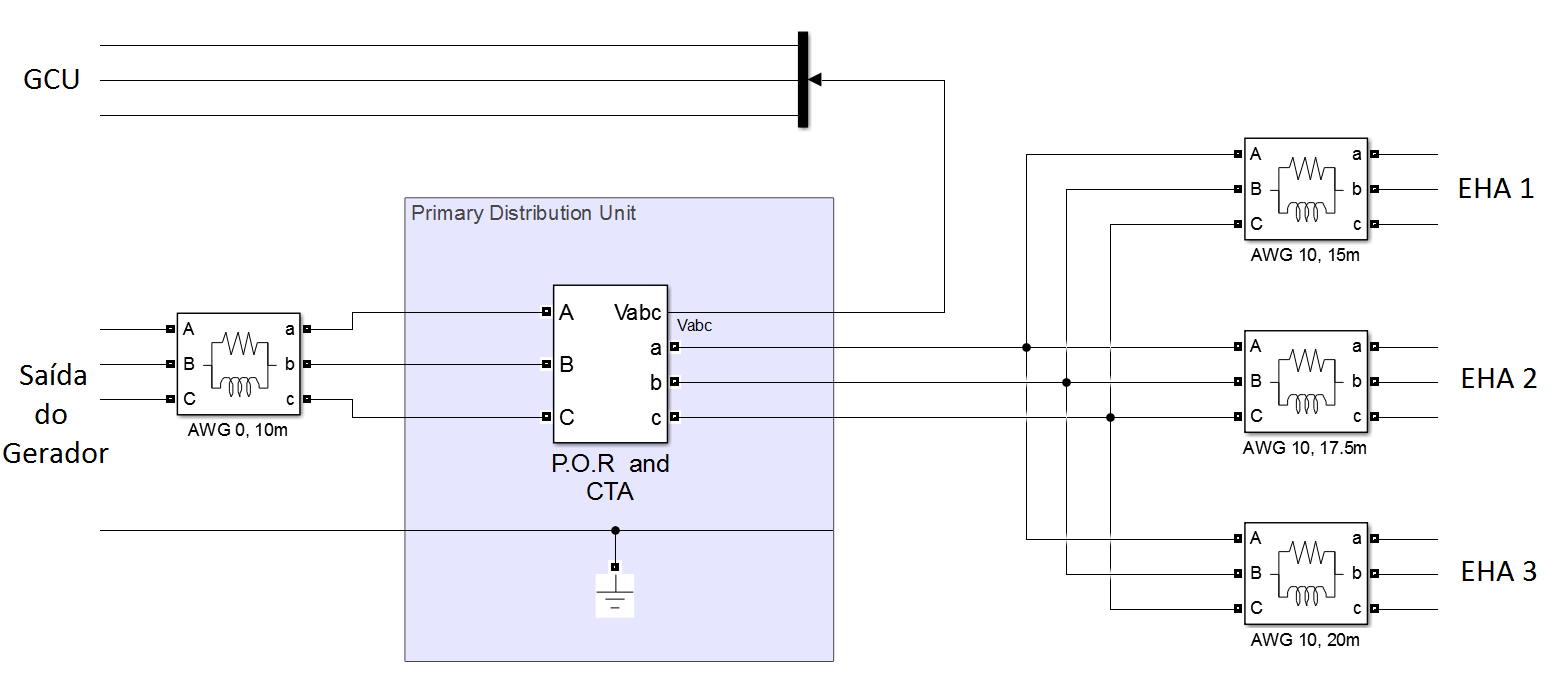
\includegraphics[width=0.99\textwidth]{Cap4/Figuras/dist.png}
	\caption{Sistema de Distribuição}
	\label{fig:dist.png}
\end{figure}

As não idealidades dos condutores são modeladas com a inserção de resistências e reatâncias indutivas conectadas em série nas linhas de transmissão do sistema. As capacitâncias entre os condutores e o plano de terra não são considerados devidos sua insignificância frente à potência e o tamanho das cablagens. As bitolas dos fios e seus comprimentos estão adequadamente dimensionados para a corrente transmitida e o tamanho comumente encontrado em uma aeronave do porte do modelo. Sendo assim, os valores de impedância de cada seção do sistema trifásico é definido seguindo os parâmetros encontrados em \cite{Exner1953}. A Tabela \ref{tab:Zdist} expõe as definições do modelo quanto às cablagens utilizadas e suas impedâncias em cada seção. 

\begin{table}[!htb]
	\centering
	\begin{tabular}{|c|c|c|c|}
		\hline
		\textbf{Porção}		&	\textbf{Bitola}		&	\textbf{Comprimento}	&	\textbf{Impedância (400 Hz) [$\Omega$]}	\\\hline
		GEN - PDU	&	AWG 0		&	10 m		&	$0,0047+j0,0067$	\\\hline
		PDU - EHA 1	&	AWG 10 		&	15 m		&	$0,0540+j0,0199$	\\\hline
		PDU - EHA 2 	&	AWG 10		&	17.5 m 		&	$0,0630+j0,0233$	\\\hline
		PDU - EHA 3	&	AWG 10		&	20 m 		&	$0,0720+j0,0266$	\\\hline
	\end{tabular}
	\caption{Impedâncias das linhas de distribuição}
	\label{tab:Zdist}
\end{table}

\subsubsection{Atuador Eletrohidrostático}

O atuador eletrohidrostático é um dispositivo empregado em sistemas de controle de voo na qual atua nas superfícies de comando para manter a aeronavegabilidade de uma aeronave. Os EHAs são compostos por dois principais subsistemas: o subsistema elétrico e o subsistema hidráulico. A porção elétrica é composta por conversores de tensão elétrica de modo a energizar um motor que impulsiona a bomba do subsistema hidráulico. Com a pressurização das linhas hidráulicas o EHA fica apto a acionar o deslocamento linear do pistão por meio da atuação de sistemas de controle.

O subsistema elétrico tem como principais componentes uma ponte trifásica de diodos, um driver DC-DC, um inversor de frequência e uma máquina síncrona baseada em imãs permanentes \cite{Dinca2014}. A Figura \ref{fig:EHA_elec.png} mostra o diagrama simplificado do subsistema elétrico. Cabe lembrar que outros componentes secundários são empregados neste subsistema com o intuito de prover controle e proteção ao EHA, e que não são mostrados na Figura \ref{fig:EHA_elec.png}.

\begin{figure}[!htb] %
	\centering
	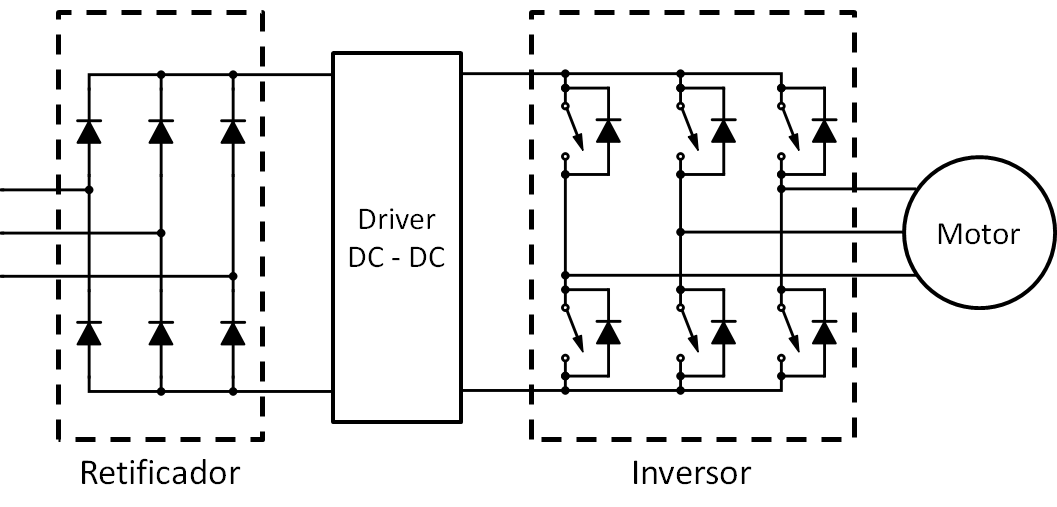
\includegraphics[width=0.7\textwidth]{Cap4/Figuras/EHA_elec.png}
	\caption{Subsistema elétrico de um EHA}
	\label{fig:EHA_elec.png}
\end{figure}  

Por apresentar uma ponte de retificadora de diodos na entrada, a operação de um EHA acaba por injetar componentes harmônicos nas formas de onda de corrente, trazendo assim a depreciação da qualidade de energia elétrica de uma aeronave. Como o foco deste trabalho diz respeito à qualidade de energia, tanto a modelagem do subsistema hidráulico juntamente com a operação do motor elétrico não será modelada. Sendo assim, o foco recai nas formas de onda da corrente que atravessam o retificador de entrada, a qual é o principal componente responsável pela queda na qualidade de energia quando se opera o EHA. A Figura \ref{fig:EHA.png} mostra o modelo do EHA empregado no Simulink para realização da simulação. Este modelo é composto por uma ponte retificadora trifásica que estabelece a conversão AC-DC, como em um EHA, sendo que no lado DC existe uma fonte de corrente controlada. A realização desta fonte tem como objetivo simular o comportamento de consumo de energia proferido pelo restante dos componentes do lado DC do subsistema elétrico. A presença de uma resistência \textit{snubber} em paralelo à fonte de corrente visa eliminar incompatibilidades do modelo, visto que isto é uma exigência para compilação do Simulink. Contudo, o valor de $R$ é escolhido com alto valor de resistência de maneira que este interfere insignificantemente ao sistema.

\begin{figure}[!htb] %
	\centering
	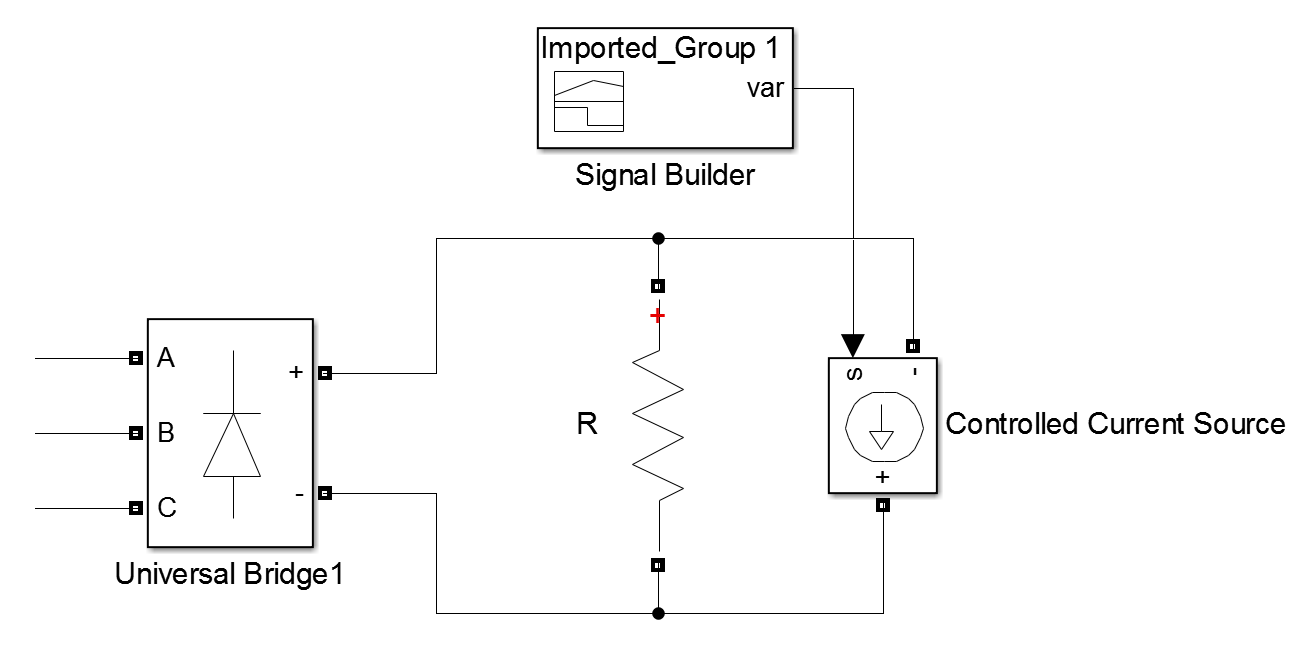
\includegraphics[width=0.7\textwidth]{Cap4/Figuras/EHA.png}
	\caption{Modelo do EHA empregado no Simulink}
	\label{fig:EHA.png}
\end{figure}

O sinal de controle da fonte de corrente do lado DC é realizado de maneira a providenciar adequadamente o consumo de corrente visto pelo lado AC de um EHA. Tal sinal de controle foi gerado utilizando resultados experimentais de um EHA operando com carga em seu pistão. A metodologia empregada para a obtenção do sinal de controle da fonte de corrente foi através do cálculo da potência aparente consumida de um EHA real, através de dados experimentais, e inferir essa mesma potência no lado DC do EHA do modelo. Com isso garante-se que a potência aparente apresentada no modelo seja a mesma de um EHA real operando com carga, além de garantir a equivalência das formas de onda da corrente no lado AC. Com essa metodologia empregada o sinal criado para o controle da fonte de corrente do lado DC do modelo é visto na Figura \ref{fig:corrente_controlada_EHA.eps}.

\begin{figure}[!htb] %
	\centering
	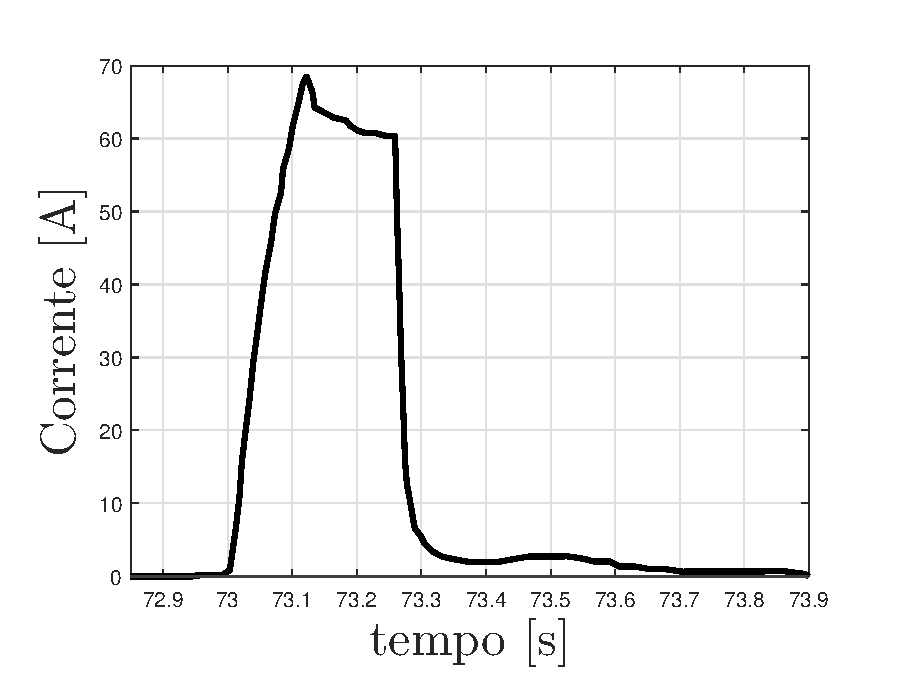
\includegraphics[width=0.7\textwidth]{Cap4/Figuras/corrente_controlada_EHA.eps}
	\caption{Valores estipulados na fonte de corrente controlada}
	\label{fig:corrente_controlada_EHA.eps}
\end{figure}

\todo{Padronizar as figuras (plots\_EHA\_teste.mat)}

\subsection{Modelo do Filtro Ativo}

O filtro ativo modelado em ambiente Simulink tem como objetivo simular a operação do controle do compensador de maneira suficientemente adequada para avaliar a eficácia da filtragem e seu emprego no setor aeronáutico. Com isso, as diversas características que viabilizam o emprego desse tipo de filtro podem ser analisadas.

O modelo é composto por diversos blocos criados para cada função constituinte de um filtro. A teoria de potência instantânea apresentadas no capítulo \ref{cap:Filtros Ativos para Sistemas Elétricos} será implementada em um desses blocos para realizar a simulação dos cálculo das correntes de referências do compensador. Já a parte relacionada com o compensador será implementado em outro bloco e segundo as definições apresentadas na seção \ref{sec:Características de Filtros Ativos em Sistemas Reais}. A operação conjunta do compensador com o controle concebe o filtro ativo como todo.

\subsubsection{Controle}

O bloco de controle visa simular os procedimentos de cálculo, os comandos dos interruptores estáticos do compensador e a malha de controle de tensão do capacitor do lado DC do inversor. Estes sub-blocos são comumente encontrados em dispositivos programáveis de sistemas reais as quais compõem um DSP.

O sub-bloco de cálculo das correntes de referência para o inversor é mostrado na Figura \ref{fig:controladador.png}. Este sub-bloco tem como entrada as tensões medidas nas linhas trifásicas do sistema elétrico no ponto anterior a conexão do filtro, e também, as correntes medidas na entrada da carga não linear, onde no caso dessa simulação é dada pelo EHA. Já a saída é composta pelas correntes de referência que alimentam o controle de comando dos interruptores do inversor estático.

O sub-bloco a qual determina as correntes de referência é constituído de duas partes, onde a porção superior (Figura \ref{fig:controladador.png}) compõe o detector de sequencia positiva, e a parte inferior constitui o cálculo das correntes de referência. A porção superior utiliza a teoria apresentada na seção \ref{subsubsec:Tipos de Controle} e estabelece os cálculos algébricos para a obtenção do sinal das tensões sem apresentar harmônicas ou componentes de sequência negativa ou zero. Este sinal é direcionado para a porção inferior, onde é utilizado com as equações da teoria da potência instantânea, discutidos no capítulo \ref{cap:Filtros Ativos para Sistemas Elétricos}, para a obtenção das correntes de referência do filtro.

\begin{figure}[!htb] %
	\centering
	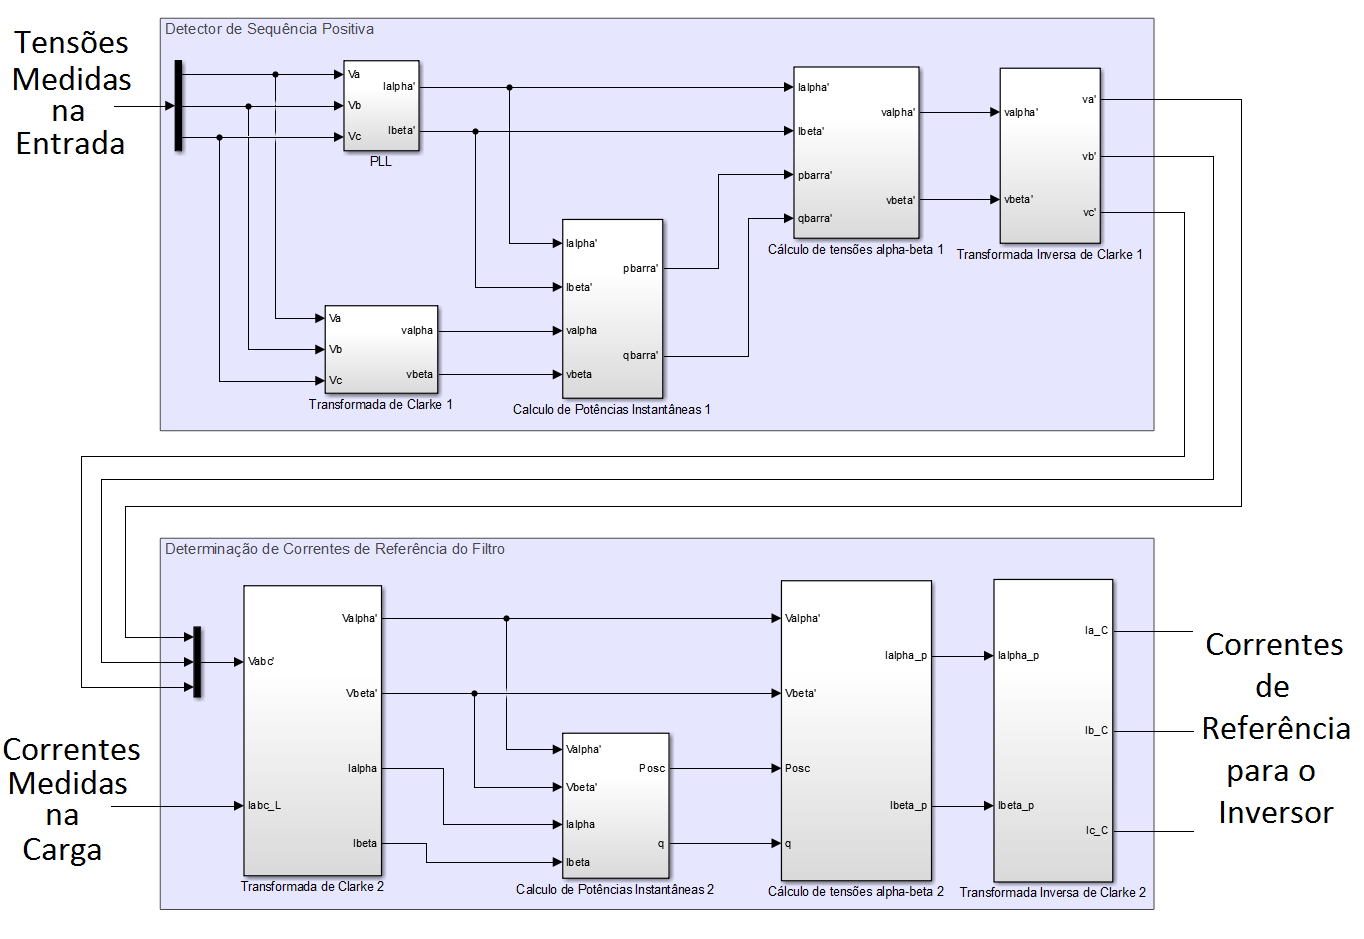
\includegraphics[width=0.99\textwidth]{Cap4/Figuras/controlador.png}
	\caption{Sub-bloco para determinação das corrente de referência}
	\label{fig:controladador.png}
\end{figure}

O sub-bloco de comando dos interruptores estáticos do inversor, onde é empregado o controle por histerese, é mostrado na Figura \ref{fig:histerese_sim.png}. Nesse bloco a entrada é composta pelos sinais de referência das correntes advindas do sub-bloco da Figura \ref{fig:controladador.png} (I\_ref), juntamente com a medição da corrente na saída do inversor (I\_meas). A saída é composta pelo sinal de comando de cada interruptor a qual é empregado no inversor.

A operação deste bloco é realizada pela comparação do sinal de referência com a medição da corrente na saída do inversor. O sinal advindo da comparação passa por um relé programado com histerese, onde é definida a banda de histerese, e por fim a saída contendo um sinal binário é gerada. Os sinais de cada fase do sistema são gerados individualmente com o controle de comutação dos interruptores de cada braço do inversor. Como estes interruptores não podem ser comutados para o estado de condução simultaneamente, seus comandos devem ser complementares. Este complemento é adquirido pela lógica NOT do sub-bloco.

\begin{figure}[!htb] %
	\centering
	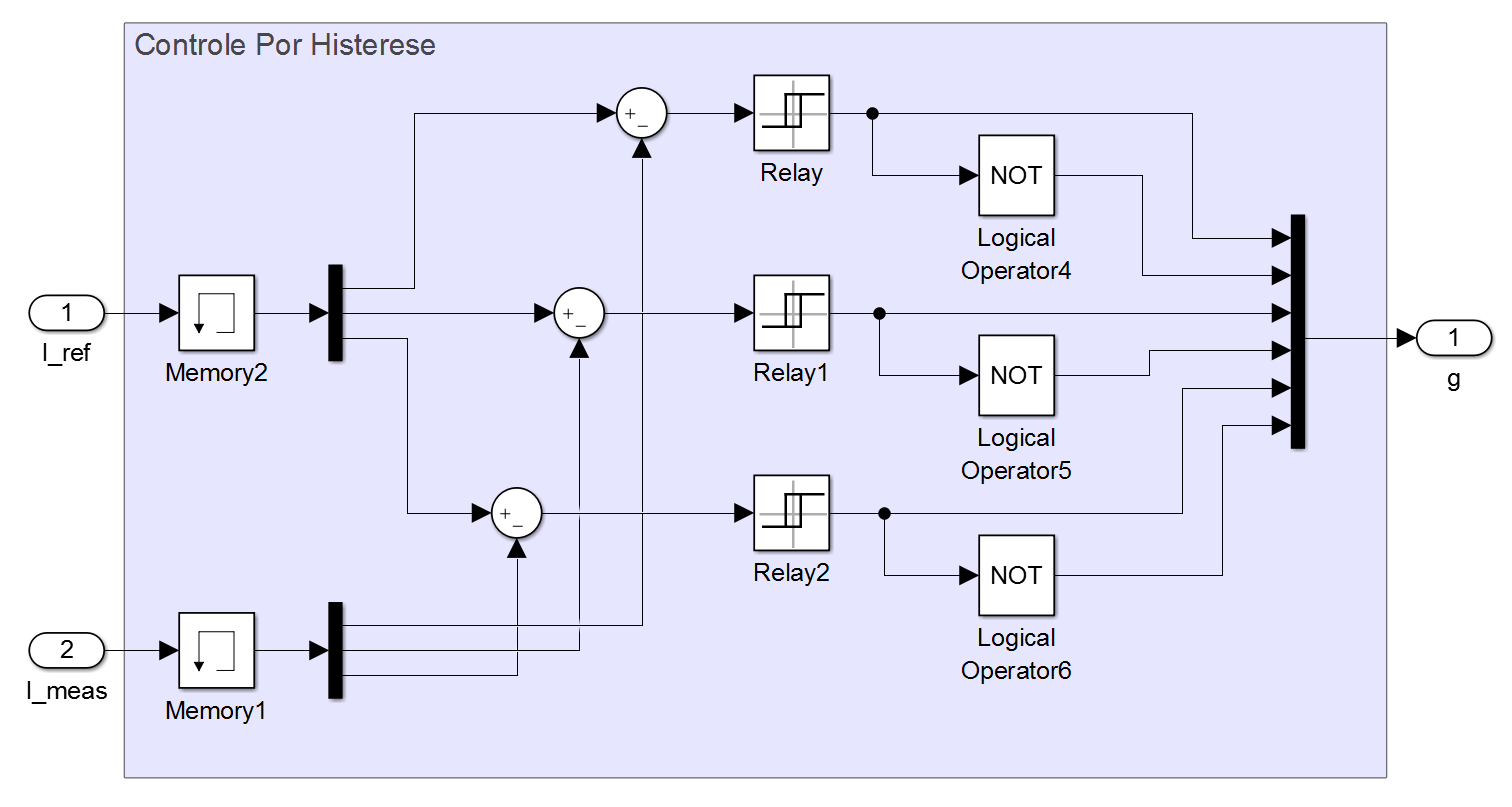
\includegraphics[width=0.7\textwidth]{Cap4/Figuras/histerese_sim.png}
	\caption{Obtenção do sinal de comando dos interruptores por controle de histerese}
	\label{fig:histerese_sim.png}
\end{figure}

O controle de tensão do capacitor disposto no lado DC do inversor é mostrado na Figura \ref{fig:PI_sim.png}. Este sub-bloco tem em sua entrada a medição de tensão do capacitor, ao passo que em sua saída é disponibilizado o sinal de potência das perdas acorridas na operação do inversor. Tal sinal de saída é direcionado para o cálculo das potências instantâneas do sub-bloco de determinação de correntes de referência (Figra \ref{fig:controladador.png}).

Este bloco constitui de um controlador proporcional-integral (PI), onde os valores de $P$ e $I$ são escolhidos de maneira a apresentar uma resposta do controlador adequada o funcionamento do sistema. A referência é obtida como um sinal degrau com amplitude fixa a qual é gerado pela \textit{Signal Builder} do Simulink. 

\begin{figure}[!htb] %
	\centering
	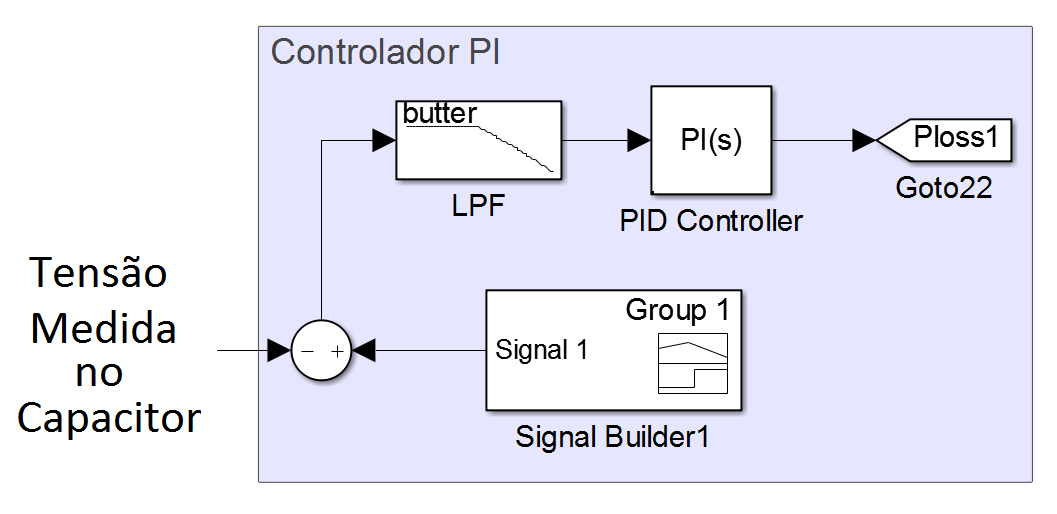
\includegraphics[width=0.5\textwidth]{Cap4/Figuras/PI_sim.png}
	\caption{Valores estipulados na fonte de corrente controlada}
	\label{fig:PI_sim.png}
\end{figure}

\subsubsection{Compensador}

O compensador criado em ambiente Simulink tem como objetivo simular a operação de um inversor composto por interruptores estáticos, nas quais são controlados pelos sinais gerados no bloco de controle para atender a demanda de corrente necessária para realização da filtragem ativa. Este bloco tem como entrada os sinais de comando dos interruptores advindos do bloco de controle por histerese. Ainda, para a correta operação do compensador algumas medições são realizadas para realimentar os sub-blocos subjacentes do modelo. Dessa maneira, a forma de onda da corrente na saída do compensador é medida para realimentar o sub-bloco de controle por histerese, e a tensão no capacitor é medida para prover seu valor ao sub-bloco de malha de controle de tensão no capacitor. Em sua saída o compensador é conectado no barramento de alimentação localizado na entrada da carga não linear, a qual conectada na rede elétrica da aeronave.

A Figura \ref{fig:Inversor.png} apresenta o bloco do compensador utilizado na simulação. Nesse bloco é empregado uma ponde de interruptores estáticos ideais ordenados como ilustrado na Figura \ref{fig:VSC.png}. A escolha dos interruptores serem estabelecidos como ideais recai na limitação do Simulink com relação às não idealidade apresentadas em elementos semicondutores de comutação. Nessa figura ainda pode ser observado a presença dos indutores de acoplamento e dos filtros capacitivos anteriores a saída do compensador. Os valores das indutâncias de acoplamento foram escolhidos subjetivamente em função da resposta estabelecida do filtro. Os valores da capacitância foram feito da mesma maneira, porém tendo em mente que altos valores de capacitância elevam a potência aparente devido ao deslocamento entre as formas de onda de tensão e corrente. Outros elementos que foram adicionados para manter a estabilidade numérica na realização da simulação são as resistências em série e em paralelo às capacitâncias. Os valores dessas resistências são escolhidos de maneira que não influem significativamente à operação do circuito, ou seja, a resistência em série e em paralelo possuem valores baixos e elevados, respectivamente.

Na Figura \ref{fig:Inversor.png} é apresentado o sub-bloco de controle por histerese para facilitar o entendimento do funcionamento do inversor.
 
\begin{figure}[!htb] %
	\centering
	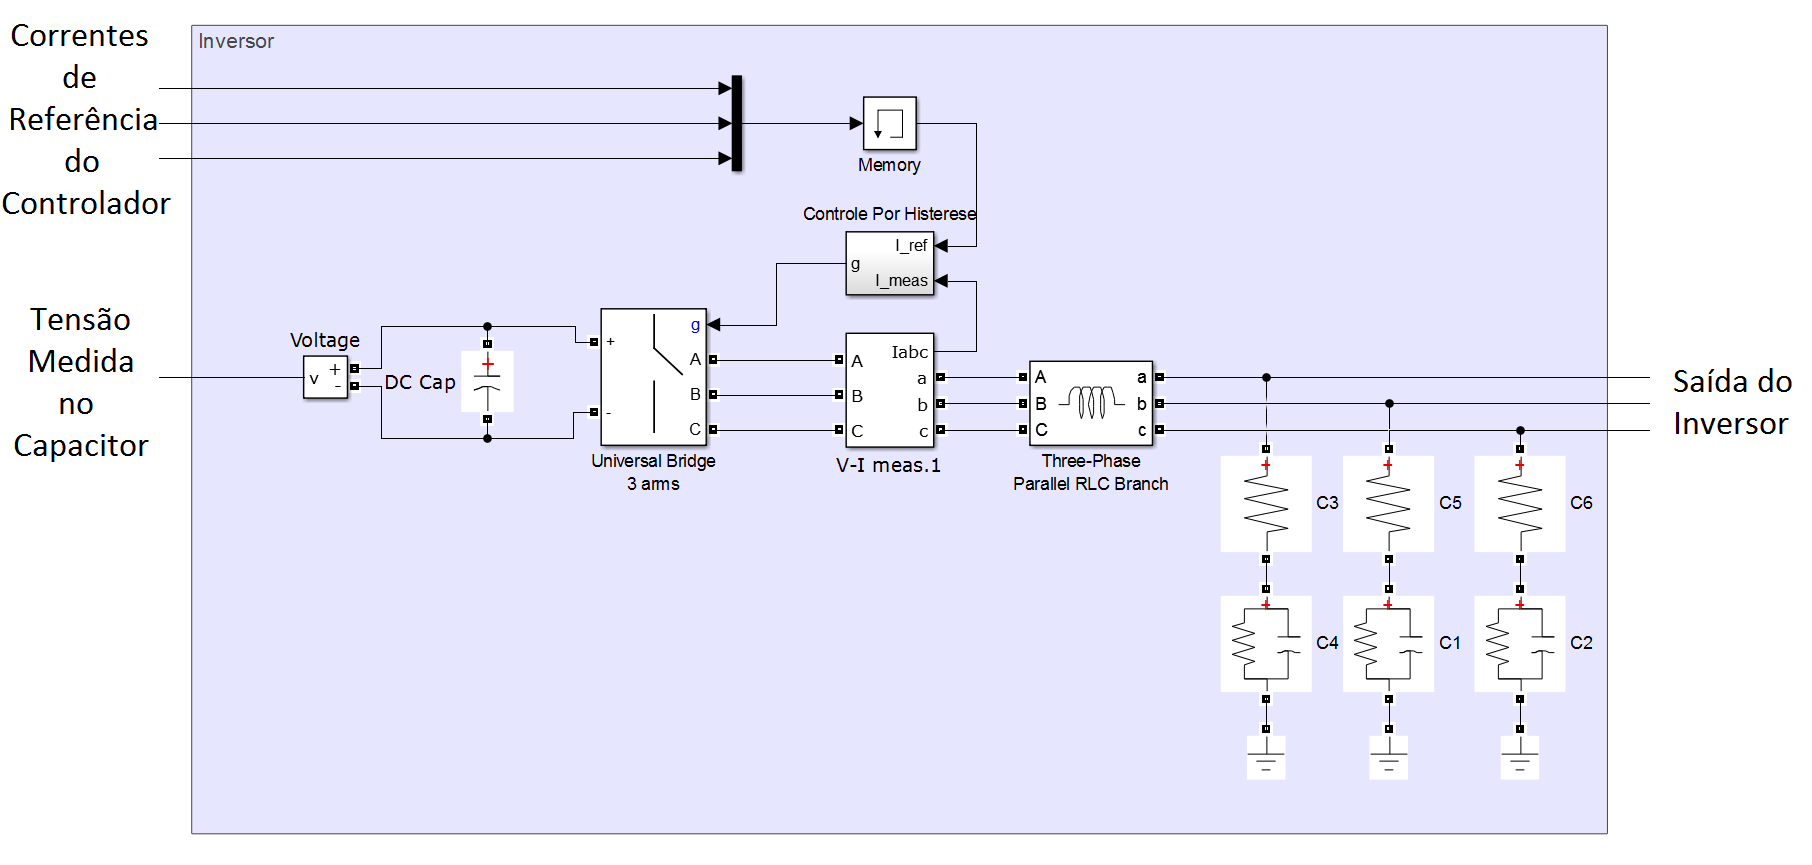
\includegraphics[width=0.99\textwidth]{Cap4/Figuras/Inversor.png}
	\caption{Valores estipulados na fonte de corrente controlada}
	\label{fig:Inversor.png}
\end{figure}

\subsection{Resultados}

A simulação comtempla a operação de três EHAs operando simultaneamente. O perfil de carga dos três EHA atuando concomitantemente é ilustrado na Figura \ref{fig:perfil.eps}. Essa corrente é solicitada com o deslocamento linear do atuador de uma extremidade a outra com a aplicação de carga mecânica em seu eixo.

\begin{figure}[!htb] %
	\centering
	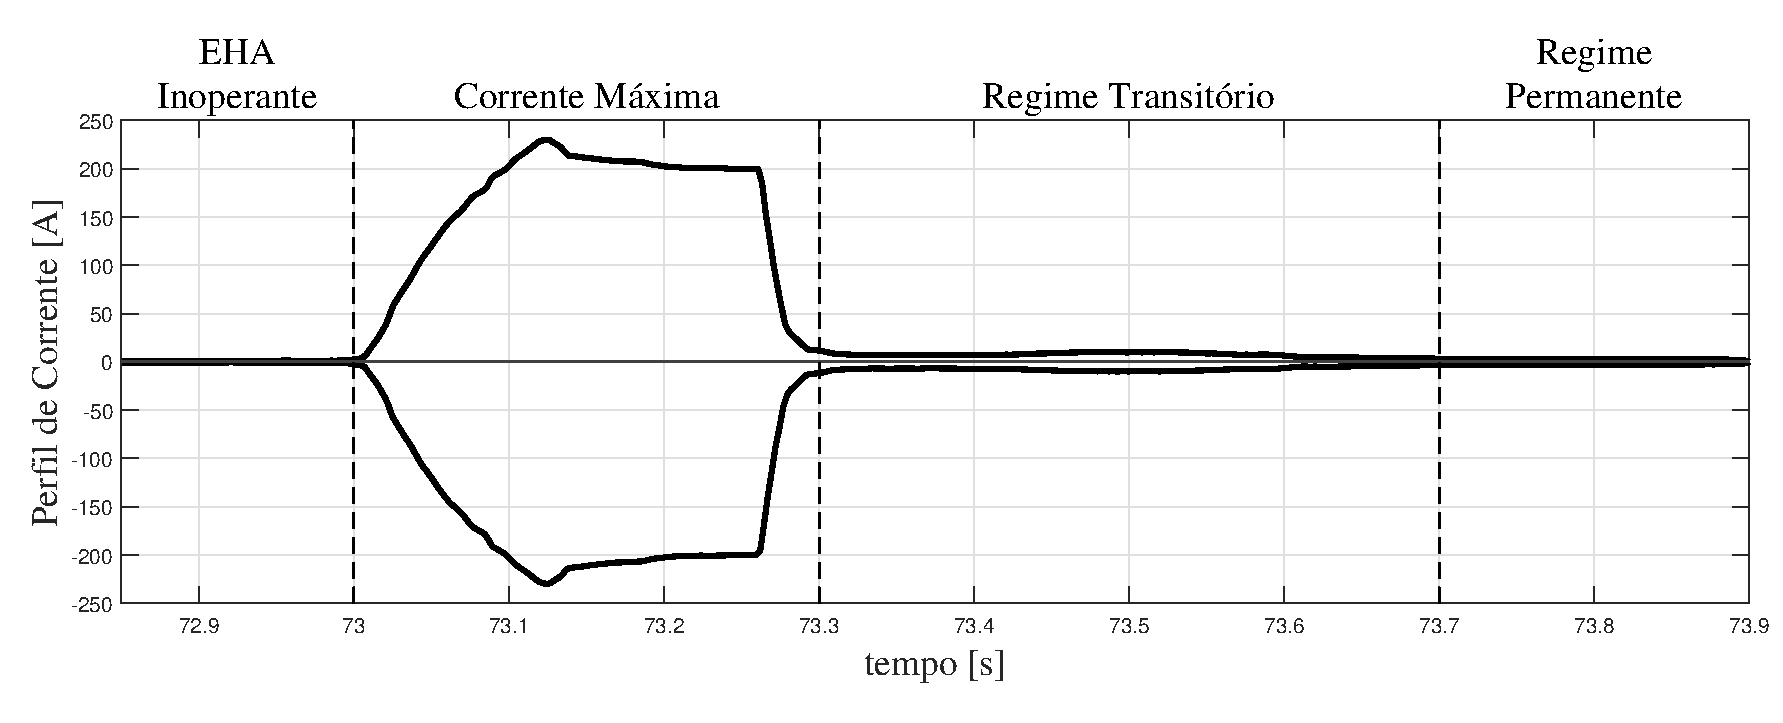
\includegraphics[width=0.99\textwidth]{Cap4/Figuras/perfil.eps}
	\caption{perfil}
	\label{fig:perfil.eps}
\end{figure}

Nesta figura pode-se observar que durante o acionamento do EHA existe uma grande variação de corrente sendo solicitada pelo atuador. Com isso, para analisar de melhor maneira o comportamento do sistema com e sem a presença do filtro ativo, a analise foi dividida em quatro principais períodos, sendo estes:

\begin{itemize}
	\item EHA inoperante: não há solicitação de uso de corrente pelo motor do EHA, sendo que a corrente apresentada é referente à fuga nos semicondutores da ponte retificadora do EHA;
	\item Corrente máxima: Período onde existe a máxima extração de corrente do sistema, onde existe à partida do motor elétrico do atuador;
	\item Regime transitório: período com oscilação de corrente após o período de máxima corrente.
	\item Regime permanente: Período sem oscilação, mas com certa corrente sendo extraída do sistema de geração.
\end{itemize}

O objetivo de dividir o período em quatro é realizado para estudar as características de operação de um filtro em períodos em que a variação da corrente solicitada pelos três EHAs varia abruptamente, sendo possível verificar o atendimento às propriedades na execução do filtro ativo tal como apresentadas no capítulo \ref{cap1}. Além disso, a visualização da análise é facilitada pela divisão, dada a grande discrepância entre os valores da corrente observado no período de corrente máxima com outros períodos.

Os resultados da simulação apresentados nas próximas seções são referentes às formas de ondas das tensões e correntes medidos na PDU, onde é avaliado a corrente que alimenta os EHAs, além da tensão de alimentação do barramento. Além disso, é realizado o cálculo das potências instantâneas em função do tempo nesse ponto. Ainda, para avaliar a condição da qualidade de energia na PDU é realizado o cálculo do espectro de frequência da tensão, cujo intuito é de comparar o resultado com as normas aeronáuticas. A norma em questão seguida como referência é a MIL-STD 704F \cite{MILSTD}, a qual propõe um limite para as distorções em função da frequência, além de restringir o TDH. Cabe a observação que os espectros de frequência presentes nesse trabalho ilustram o pico de tensão da fundamental. Esse pico é estabelecido em 400 Hz e deve ser desconsiderado na análise de qualidade de energia.

A apresentação das figuras seguintes está disposta com os resultados lado a lado com e sem a atuação do filtro ativo para efeito de comparação. As figuras localizadas no lado esquerdo são referentes ao sistema sem o filtro ativo, ao passo que as do lado direito são com a presença do filtro ativo.

\subsubsection{EHA Inoperante}

Durante o período entre 72,85 e 73 segundos o EHA não é solicitado a atuar, isto é, a corrente presente no lado DC do conversor de entrada do EHA é estabelecida apenas pela presença do resistor em paralelo com a fonte de corrente controlada. 

A Figura \ref{fig:2} apresenta as tensões e correntes medidas na PDU em um pequeno intervalo desse período. Aqui pode ser observado que na ausência do filtro ativo (Figura \ref{fig:resultados_unfilt_2.eps}) a corrente contemplada é irrelevante, dado que esta é devido apenas pela presença do resistor em paralelo com a fonte controlada. Todavia, para o caso onde há aplicação do filtro ativo (Figura \ref{fig:resultados_filt_2.eps}) um ruído intenso é medido na corrente da PDU. Isto se deve à comutação dos semicondutores do inversor do filtro ativo. Nesse caso, por não haver uma solicitação de fornecimento de corrente, o filtro apresenta esse comportamento e o ruído de corrente apresenta-se relevante frente a ausência do filtro. Ainda, pela analise da Figura \ref{fig:4}, onde é ilustrado as potências instantâneas medidas com as tensões e corrente na PDU, a presença do filtro ativo (Figura \ref{fig:resultados_unfilt_4.eps}) deixa as potências igualmente ruidosas.

Os espectros de frequência podem ser analisados nas figuras \ref{fig:5} e \ref{fig:6}. Aqui pode ser observado que a presença do filtro ativo deteriora a qualidade de energia, porém os níveis de tensão do espectro e o THD está sempre presente dentro dos limites da MIL-STD 704F. 

%\begin{figure*}[!htb] %Circuito típico de um retificador de 12 pulsos com sua respectiva corrente de entrada
%	\centering
%	\begin{subfigure}[b]{0.48\textwidth}
%		\centering
%		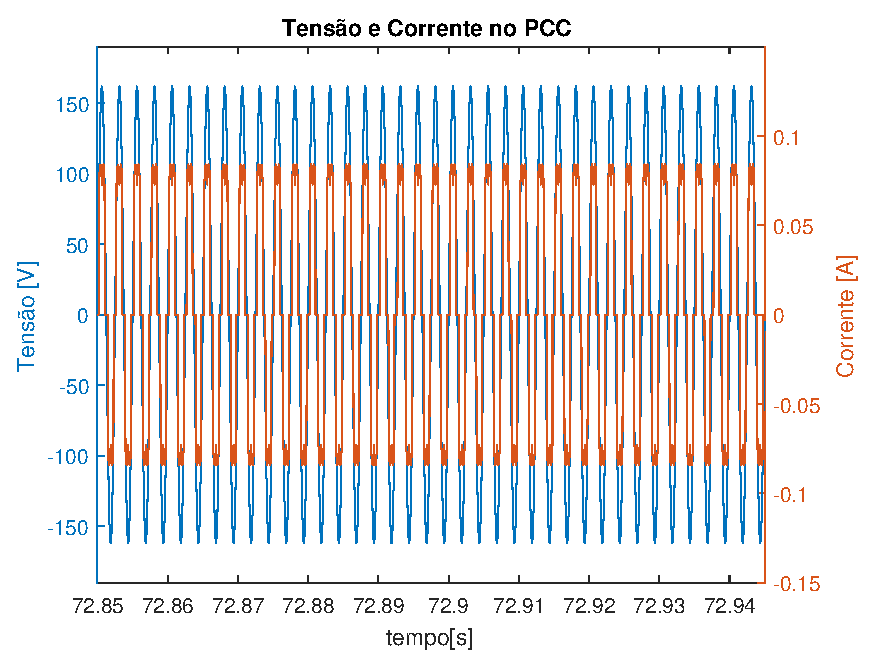
\includegraphics[width=\textwidth]{Cap4/Figuras/resultados_unfilt_1.eps}
%		\caption{Topologia típica de um VSC} 
%		\label{fig:VSC.png}
%	\end{subfigure}%
%		\hfill
%	\begin{subfigure}[b]{0.48\textwidth}  
%		\centering 
%		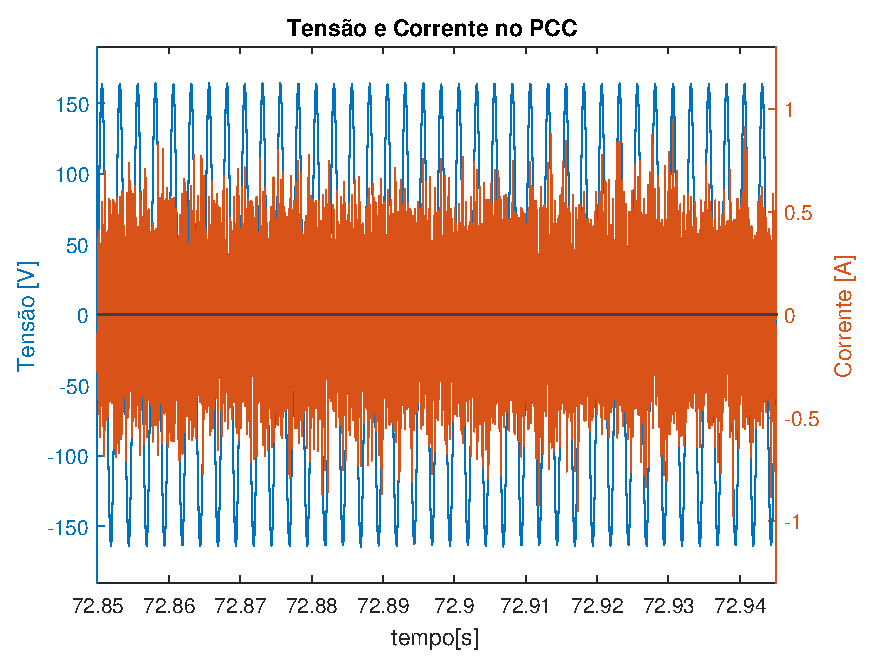
\includegraphics[width=\textwidth]{Cap4/Figuras/resultados_filt_1.eps}
%		\caption{Topologia típica de um CSC}    
%		\label{fig:CSC.png}
%	\end{subfigure}%
%	\caption{1}
%	\label{fig:1}
%\end{figure*}

\begin{figure*}[!htb] %Circuito típico de um retificador de 12 pulsos com sua respectiva corrente de entrada
	\centering
	\begin{subfigure}[b]{0.48\textwidth}
		\centering
		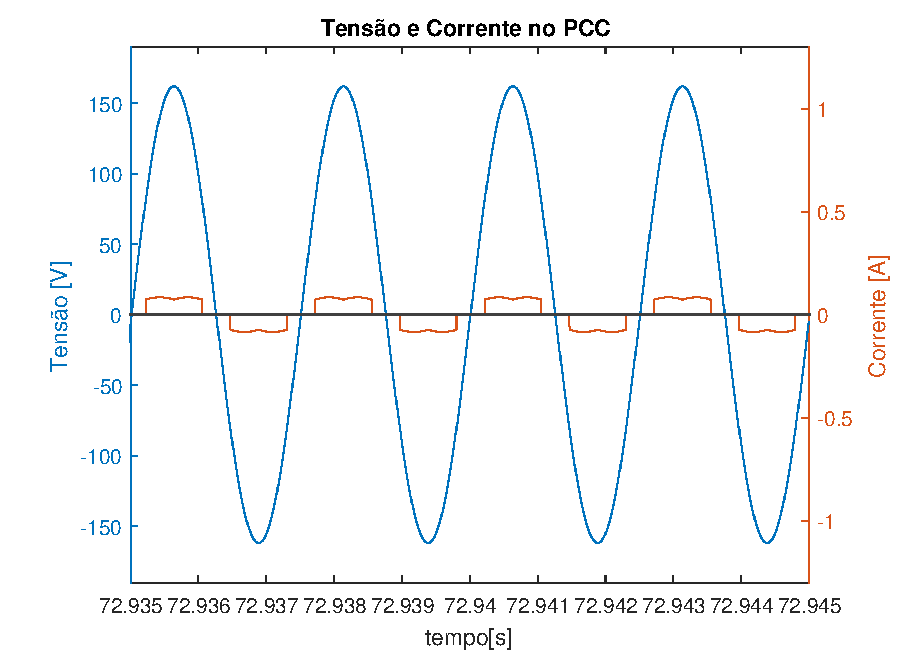
\includegraphics[width=\textwidth]{Cap4/Figuras/resultados_unfilt_2.eps}
		\caption{Topologia típica de um VSC} 
		\label{fig:resultados_unfilt_2.eps}
	\end{subfigure}%
		\hfill
	\begin{subfigure}[b]{0.48\textwidth}  
		\centering 
		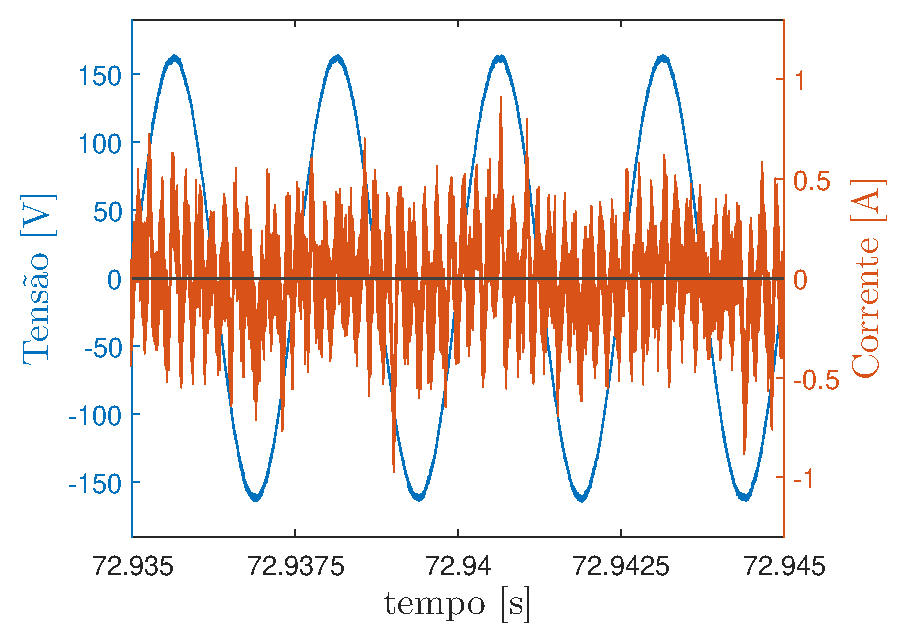
\includegraphics[width=\textwidth]{Cap4/Figuras/resultados_filt_2.eps}
		\caption{Topologia típica de um CSC}    
		\label{fig:resultados_filt_2.eps}
	\end{subfigure}%
	\caption{2}
	\label{fig:2}
\end{figure*}

%\begin{figure*}[!htb] %Circuito típico de um retificador de 12 pulsos com sua respectiva corrente de entrada
%	\centering
%	\begin{subfigure}[b]{0.48\textwidth}
%		\centering
%		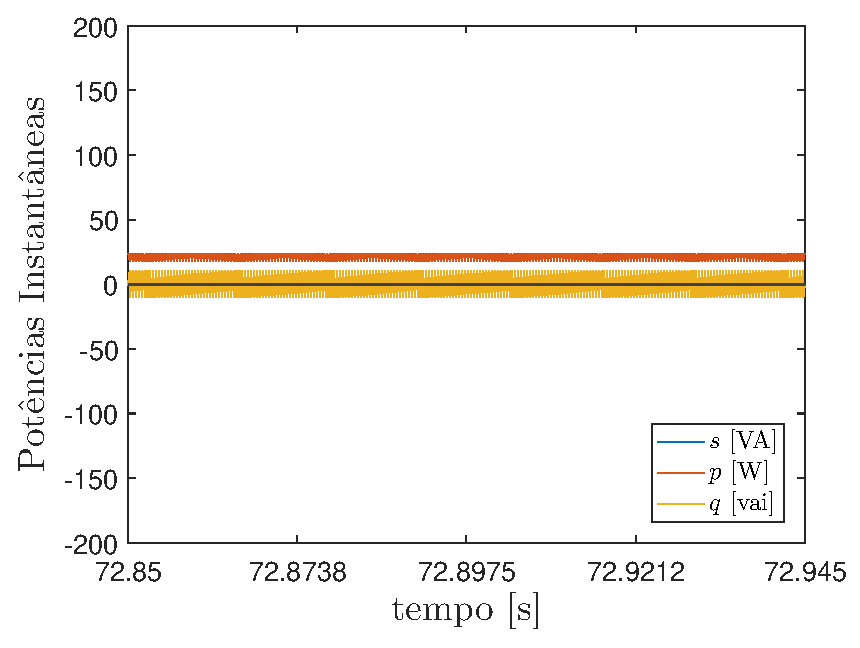
\includegraphics[width=\textwidth]{Cap4/Figuras/resultados_unfilt_3.eps}
%		\caption{Topologia típica de um VSC} 
%		\label{fig:VSC.png}
%	\end{subfigure}%
%		\hfill
%	\begin{subfigure}[b]{0.48\textwidth}  
%		\centering 
%		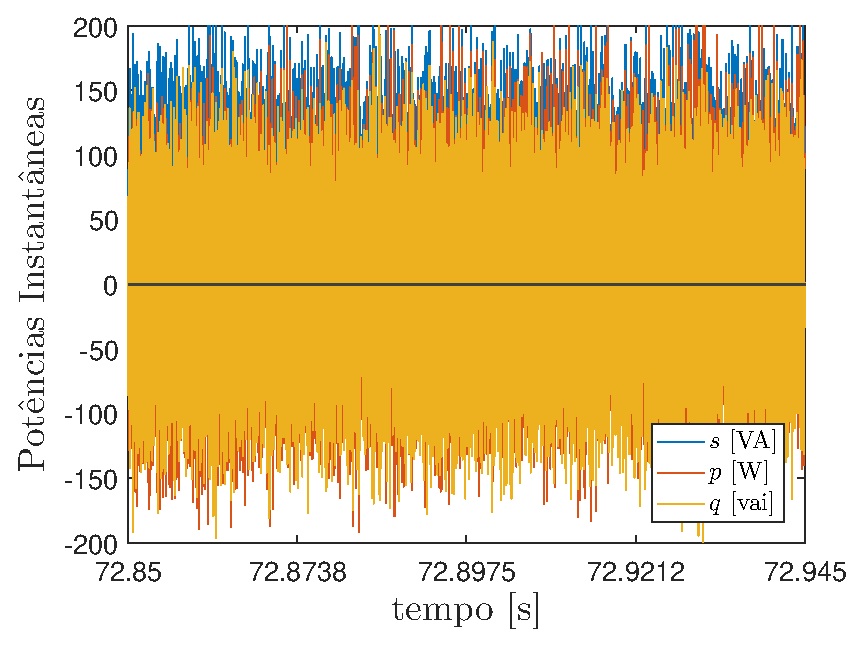
\includegraphics[width=\textwidth]{Cap4/Figuras/resultados_filt_3.eps}
%		\caption{Topologia típica de um CSC}    
%		\label{fig:CSC.png}
%	\end{subfigure}%
%	\caption{3}
%	\label{fig:3}
%\end{figure*}

\begin{figure*}[!htb] %Circuito típico de um retificador de 12 pulsos com sua respectiva corrente de entrada
	\centering
	\begin{subfigure}[b]{0.48\textwidth}
		\centering
		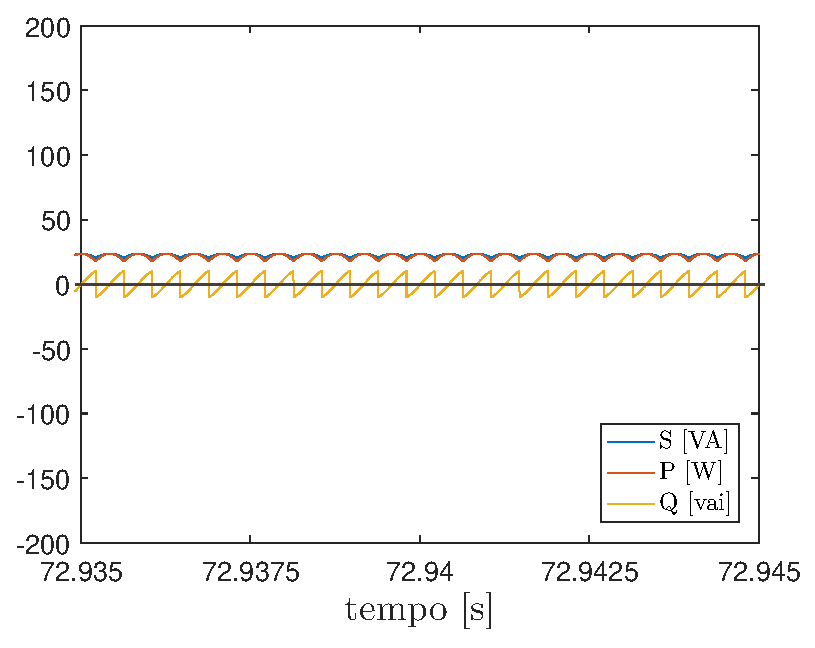
\includegraphics[width=\textwidth]{Cap4/Figuras/resultados_unfilt_4.eps}
		\caption{Topologia típica de um VSC} 
		\label{fig:resultados_unfilt_4.eps}
	\end{subfigure}%
		\hfill
	\begin{subfigure}[b]{0.48\textwidth}  
		\centering 
		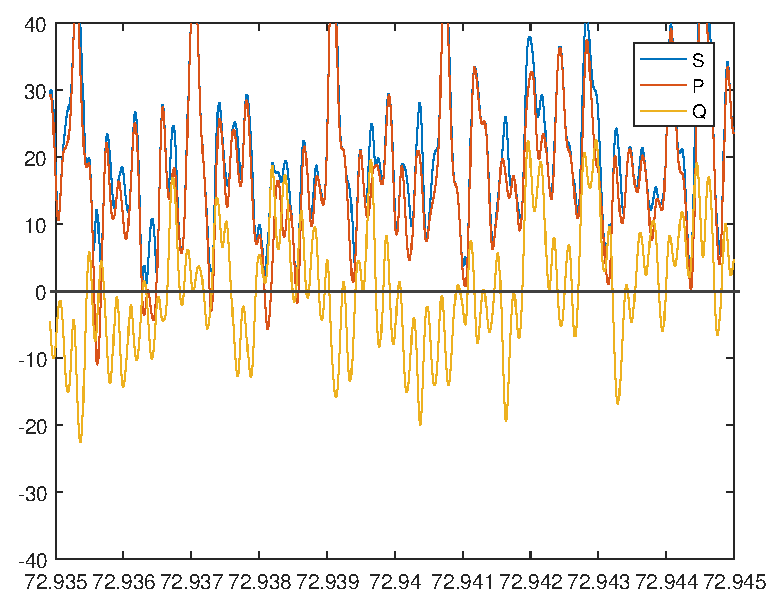
\includegraphics[width=\textwidth]{Cap4/Figuras/resultados_filt_4.eps}
		\caption{Topologia típica de um CSC}    
		\label{fig:resultados_filt_4.eps}
	\end{subfigure}%
	\caption{4}
	\label{fig:4}
\end{figure*}

\begin{figure*}[!htb] %Circuito típico de um retificador de 12 pulsos com sua respectiva corrente de entrada
	\centering
	\begin{subfigure}[b]{0.48\textwidth}
		\centering
		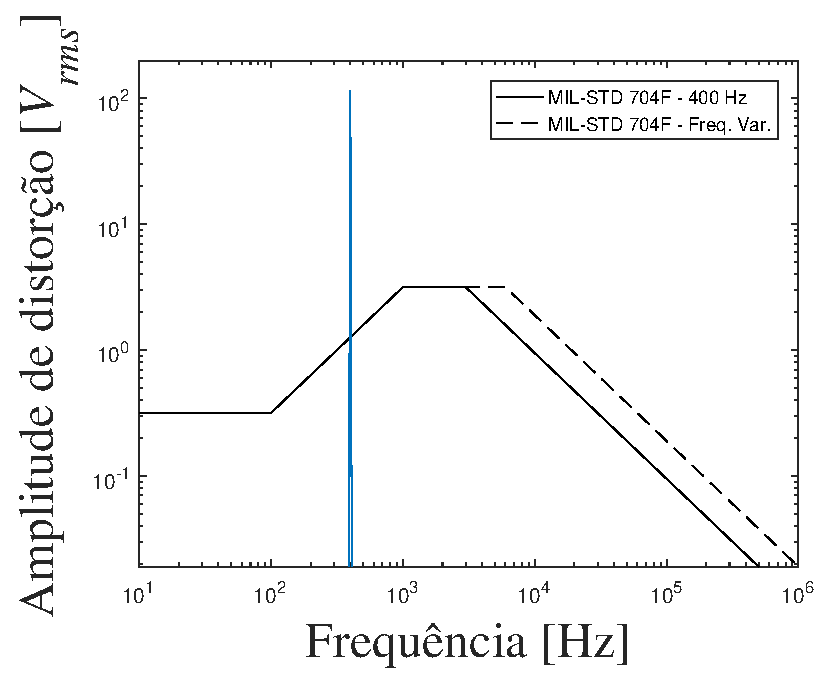
\includegraphics[width=\textwidth]{Cap4/Figuras/resultados_unfilt_5.eps}
		\caption{Topologia típica de um VSC} 
		\label{fig:resultados_unfilt_5.eps}
	\end{subfigure}%
		\hfill
	\begin{subfigure}[b]{0.48\textwidth}  
		\centering 
		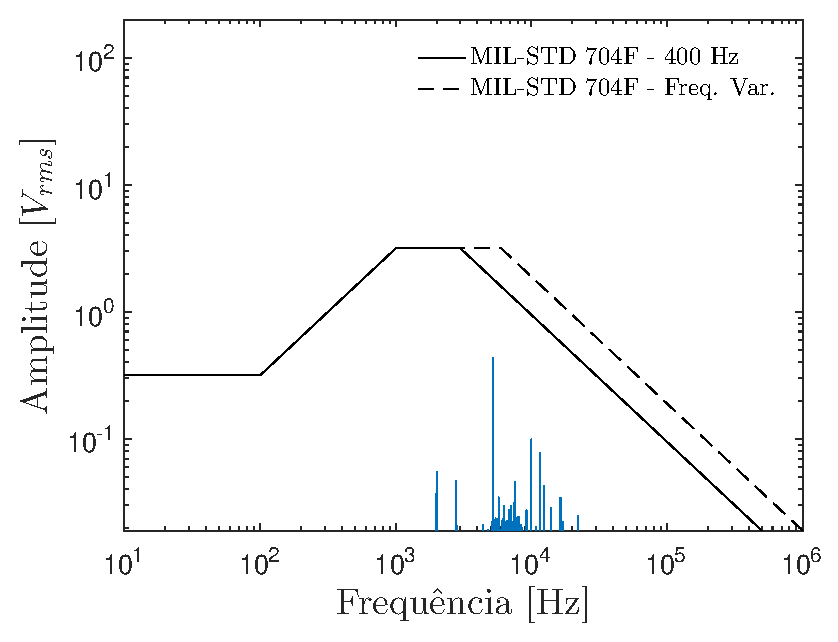
\includegraphics[width=\textwidth]{Cap4/Figuras/resultados_filt_5.eps}
		\caption{Topologia típica de um CSC}    
		\label{fig:resultados_filt_5.eps}
	\end{subfigure}%
	\caption{5}
	\label{fig:5}
\end{figure*}

\begin{figure*}[!htb] %Circuito típico de um retificador de 12 pulsos com sua respectiva corrente de entrada
	\centering
	\begin{subfigure}[b]{0.48\textwidth}
		\centering
		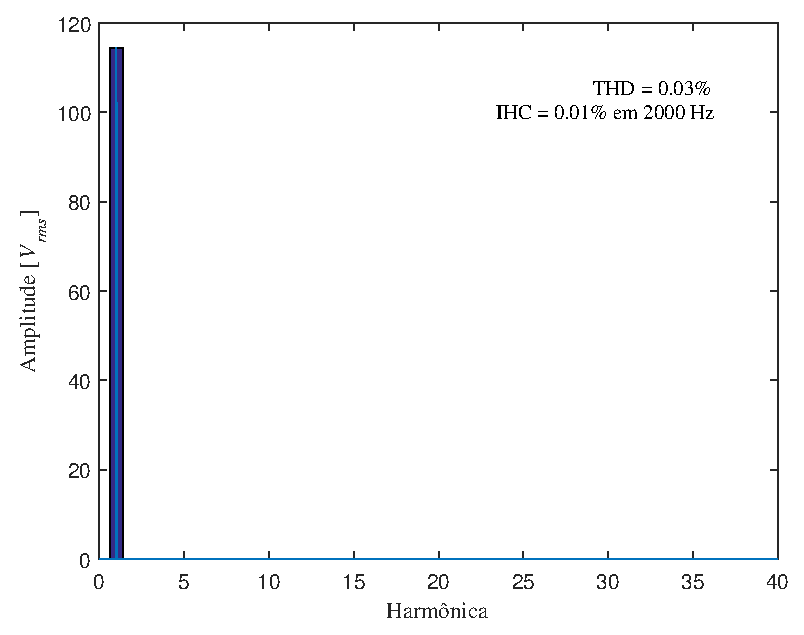
\includegraphics[width=\textwidth]{Cap4/Figuras/resultados_unfilt_6.eps}
		\caption{Topologia típica de um VSC} 
		\label{fig:resultados_unfilt_6.eps}
	\end{subfigure}%
		\hfill
	\begin{subfigure}[b]{0.48\textwidth}  
		\centering 
		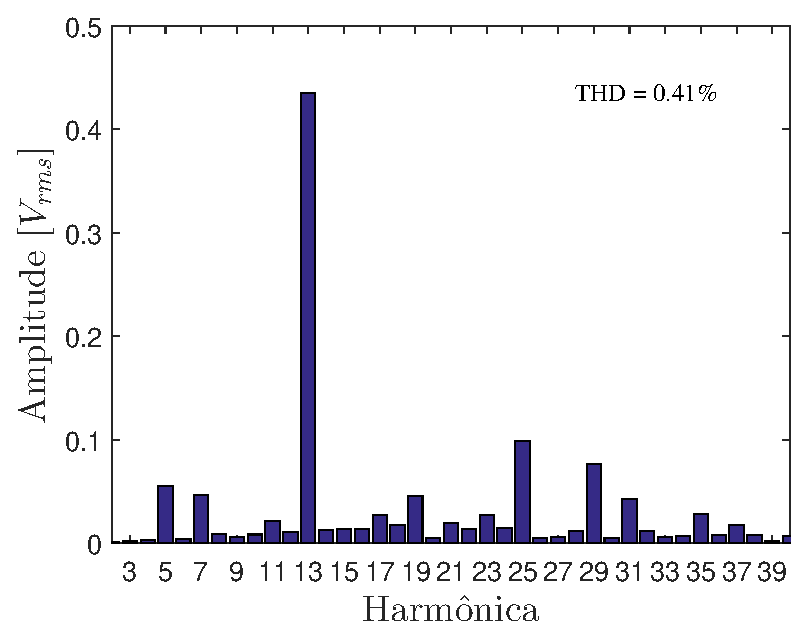
\includegraphics[width=\textwidth]{Cap4/Figuras/resultados_filt_6.eps}
		\caption{Topologia típica de um CSC}    
		\label{fig:resultados_filt_6.eps}
	\end{subfigure}%
	\caption{6}
	\label{fig:6}
\end{figure*}

\FloatBarrier

\subsubsection{Corrente Máxima}

No momento delimitado entre 73 a 73,3 é observada a corrente máxima percorrendo o sistema elétrico. A corrente nesse período é elevada devido à partida do motor elétrico, a qual exige uma corrente intensa para vencer a inercia do eixo rotativo.

A Figura \ref{fig:7} mostra as formas de onda da tensão e corrente nesse período. Por ser elevada a corrente nesse período a qualidade de energia é acentuadamente afetada. Isso pode ser na Figura \ref{fig:8}, onde é apresentado um pequeno intervalo a qual existe o pico de corrente máximo entre 73,12 e 73,13 segundos. Pela analise da Figura \ref{fig:resultados_unfilt_8.eps}, pode-se observar a forma de onda das tensões como sendo bastante distorcidas. Contudo, com a aplicação do filtro ativo pode-se observar, através da Figura \ref{fig:resultados_filt_7.eps}, que as formas de onda da corrente e da tensão são quase senoidais e em fase entre si.

A Figura \ref{fig:10} apresenta as potências instantâneas desse período. Pode-se observar que para o caso sem o filtro ativo tanto a potência ativa quanto reativa apresentam elevados valores de $\tilde{p}$ e $\tilde{q}$ respectivamente, e que são condições de baixa qualidade de energia e fator de potência. Para o caso onde o filtro ativo é presente as formas de onda das potências, apesar de apresentarem certa oscilação devido aos efeitos de comutação dos semicondutores, estão em acordo com o comportamento esperado.

Já a análise dos espectros de frequência das tensões mostra que a qualidade de energia é conseguida com a aplicação do filtro ativo. Isto é verificado pois tanto a Figura \ref{fig:resultados_unfilt_11.eps} quanto a Figura \ref{fig:resultados_unfilt_12.eps} mostram que a MIL-STD 704F não está sendo cumprida, dado que o espectro de frequência da tensão está fora dos limites da norma e o THD é superior à 5\%. Entretanto as figuras \ref{fig:resultados_filt_11.eps} e \ref{fig:resultados_filt_12.eps} apresentam a tensão na PDU dentro das especificações da MIL-STD 704F.

\begin{figure*}[!htb] %Circuito típico de um retificador de 12 pulsos com sua respectiva corrente de entrada
	\centering
	\begin{subfigure}[b]{0.48\textwidth}
		\centering
		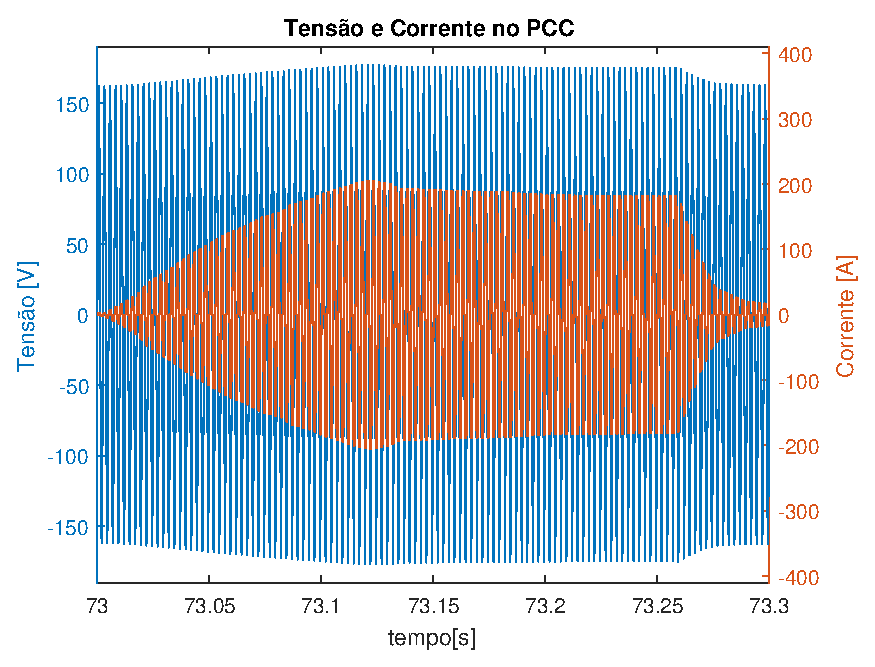
\includegraphics[width=\textwidth]{Cap4/Figuras/resultados_unfilt_7.eps}
		\caption{Topologia típica de um VSC} 
		\label{fig:resultados_unfilt_7.eps}
	\end{subfigure}%
		\hfill
	\begin{subfigure}[b]{0.48\textwidth}  
		\centering 
		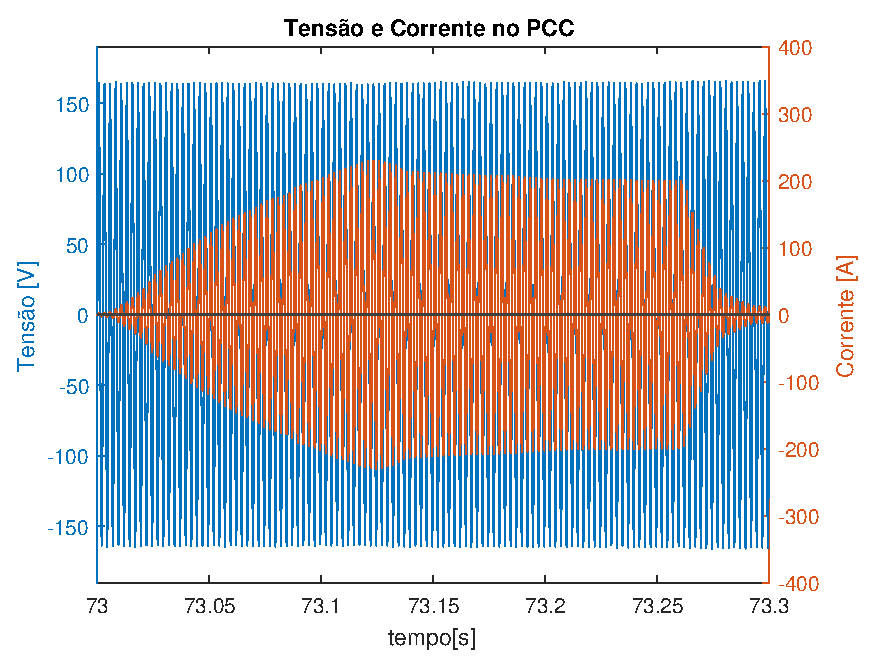
\includegraphics[width=\textwidth]{Cap4/Figuras/resultados_filt_7.eps}
		\caption{Topologia típica de um CSC}    
		\label{fig:resultados_filt_7.eps}
	\end{subfigure}%
	\caption{7}
	\label{fig:7}
\end{figure*}

\begin{figure*}[!htb] %Circuito típico de um retificador de 12 pulsos com sua respectiva corrente de entrada
	\centering
	\begin{subfigure}[b]{0.48\textwidth}
		\centering
		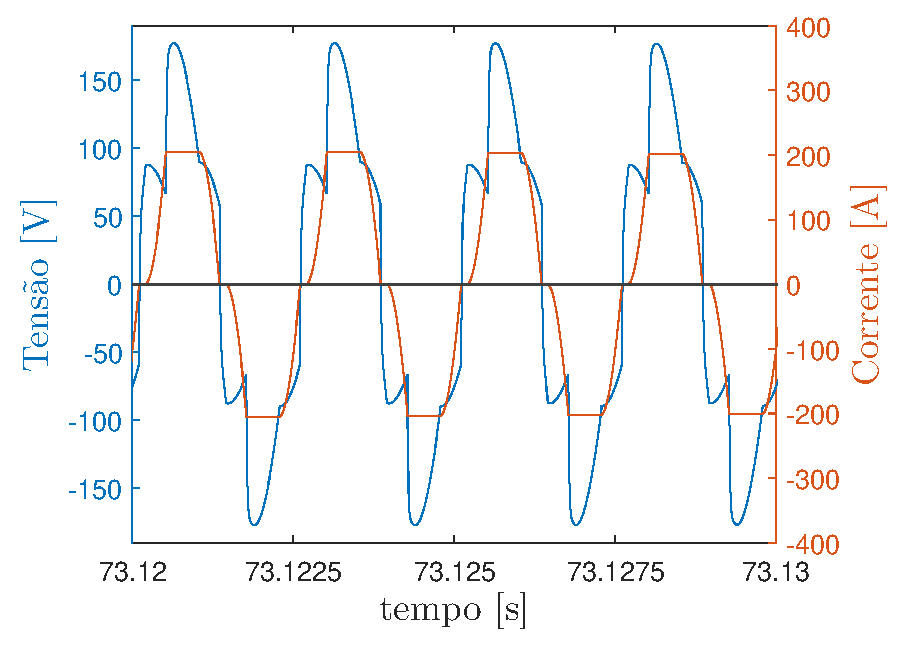
\includegraphics[width=\textwidth]{Cap4/Figuras/resultados_unfilt_8.eps}
		\caption{Topologia típica de um VSC} 
		\label{fig:resultados_unfilt_8.eps}
	\end{subfigure}%
		\hfill
	\begin{subfigure}[b]{0.48\textwidth}  
		\centering 
		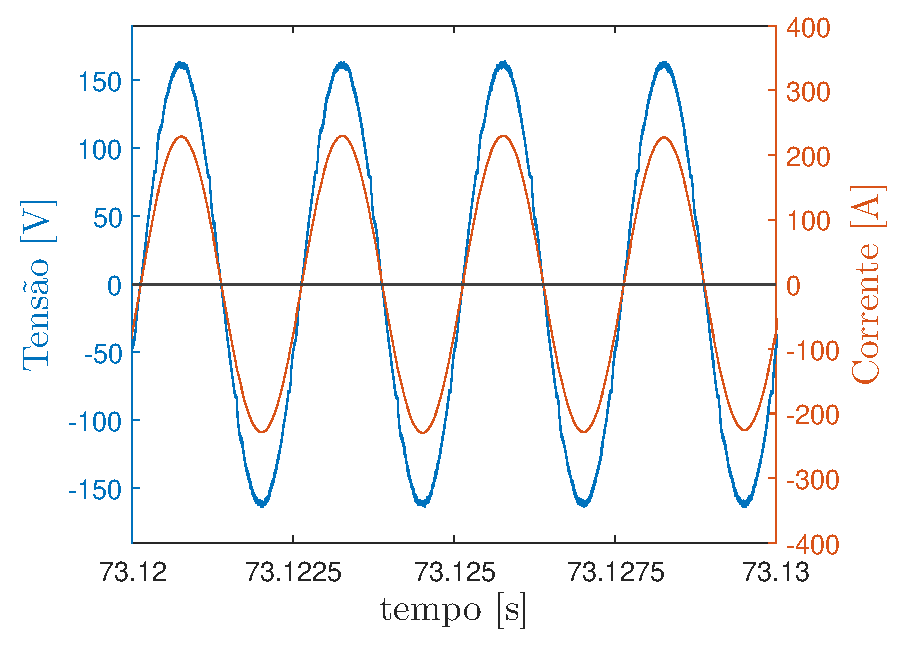
\includegraphics[width=\textwidth]{Cap4/Figuras/resultados_filt_8.eps}
		\caption{Topologia típica de um CSC}    
		\label{fig:resultados_filt_8.eps}
	\end{subfigure}%
	\caption{8}
	\label{fig:8}
\end{figure*}

\begin{figure*}[!htb] %Circuito típico de um retificador de 12 pulsos com sua respectiva corrente de entrada
	\centering
	\begin{subfigure}[b]{0.48\textwidth}
		\centering
		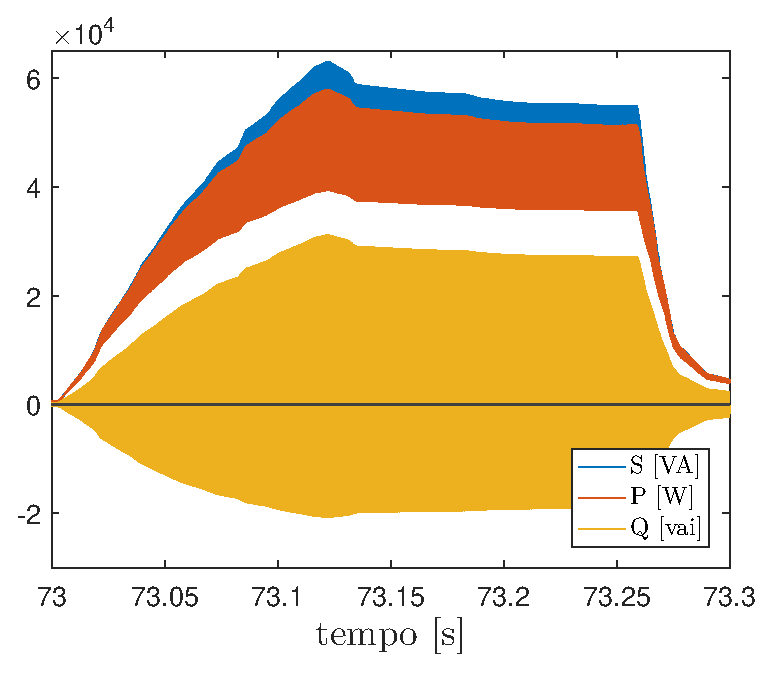
\includegraphics[width=\textwidth]{Cap4/Figuras/resultados_unfilt_9.eps}
		\caption{Topologia típica de um VSC} 
		\label{fig:resultados_unfilt_9.eps}
	\end{subfigure}%
		\hfill
	\begin{subfigure}[b]{0.48\textwidth}  
		\centering 
		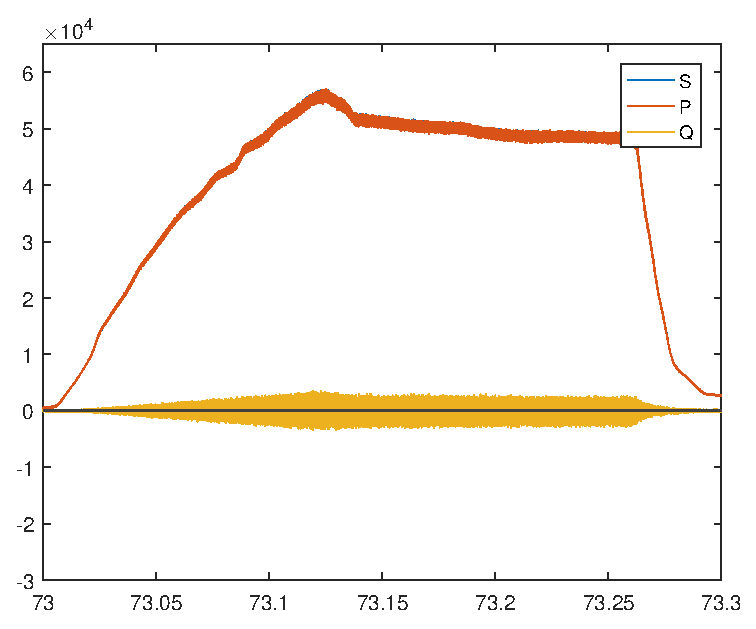
\includegraphics[width=\textwidth]{Cap4/Figuras/resultados_filt_9.eps}
		\caption{Topologia típica de um CSC}    
		\label{fig:resultados_filt_9.eps}
	\end{subfigure}%
	\caption{9}
	\label{fig:9}
\end{figure*}

\begin{figure*}[!htb] %Circuito típico de um retificador de 12 pulsos com sua respectiva corrente de entrada
	\centering
	\begin{subfigure}[b]{0.48\textwidth}
		\centering
		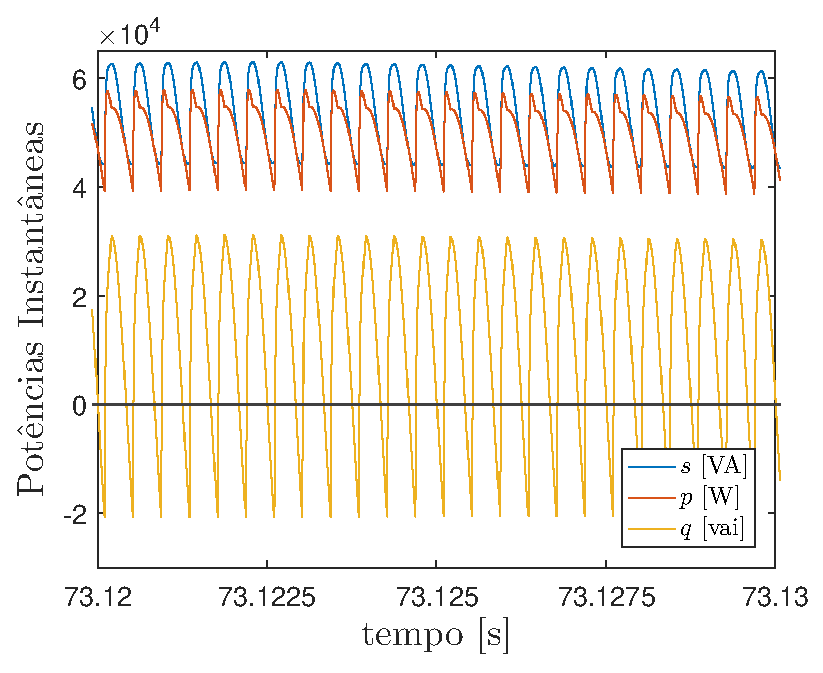
\includegraphics[width=\textwidth]{Cap4/Figuras/resultados_unfilt_10.eps}
		\caption{Topologia típica de um VSC} 
		\label{fig:resultados_unfilt_10.eps}
	\end{subfigure}%
		\hfill
	\begin{subfigure}[b]{0.48\textwidth}  
		\centering 
		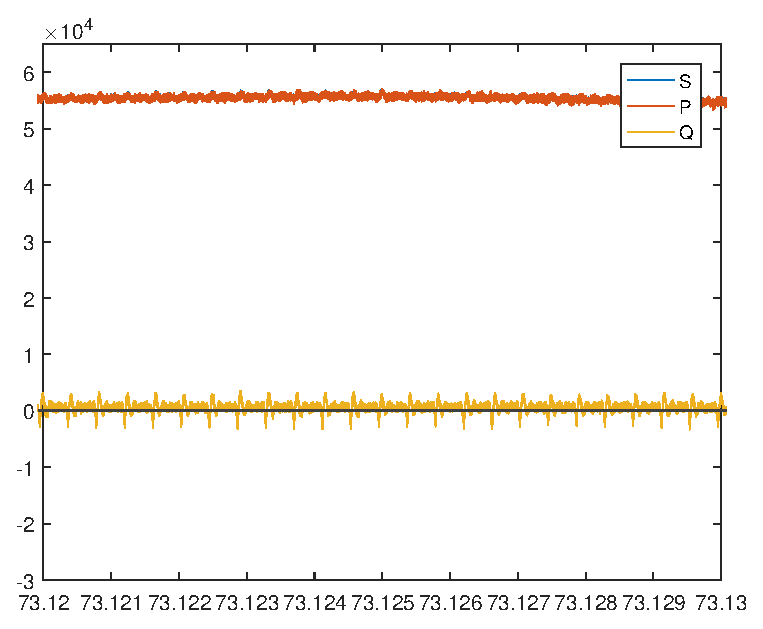
\includegraphics[width=\textwidth]{Cap4/Figuras/resultados_filt_10.eps}
		\caption{Topologia típica de um CSC}    
		\label{fig:resultados_filt_10.eps}
	\end{subfigure}%
	\caption{10}
	\label{fig:10}
\end{figure*}

\begin{figure*}[!htb] %Circuito típico de um retificador de 12 pulsos com sua respectiva corrente de entrada
	\centering
	\begin{subfigure}[b]{0.48\textwidth}
		\centering
		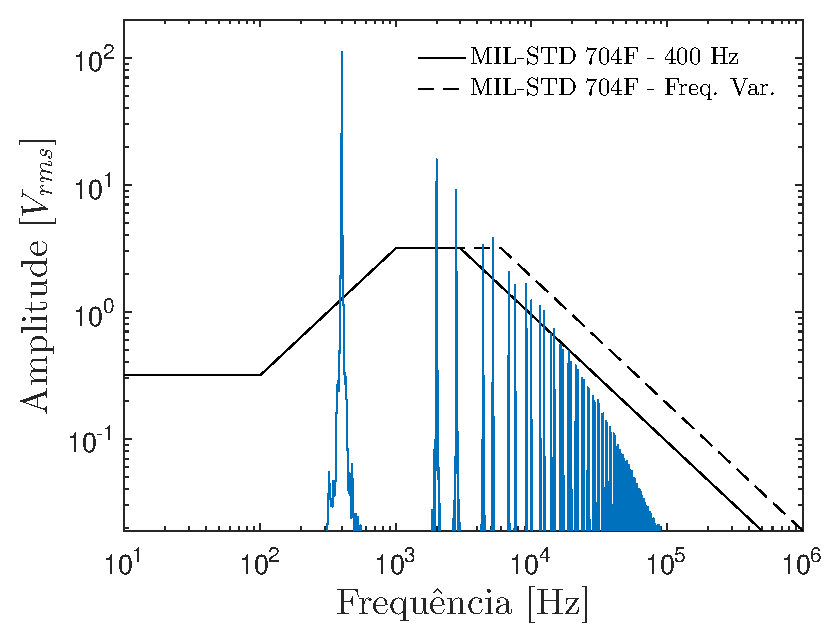
\includegraphics[width=\textwidth]{Cap4/Figuras/resultados_unfilt_11.eps}
		\caption{Topologia típica de um VSC} 
		\label{fig:resultados_unfilt_11.eps}
	\end{subfigure}%
		\hfill
	\begin{subfigure}[b]{0.48\textwidth}  
		\centering 
		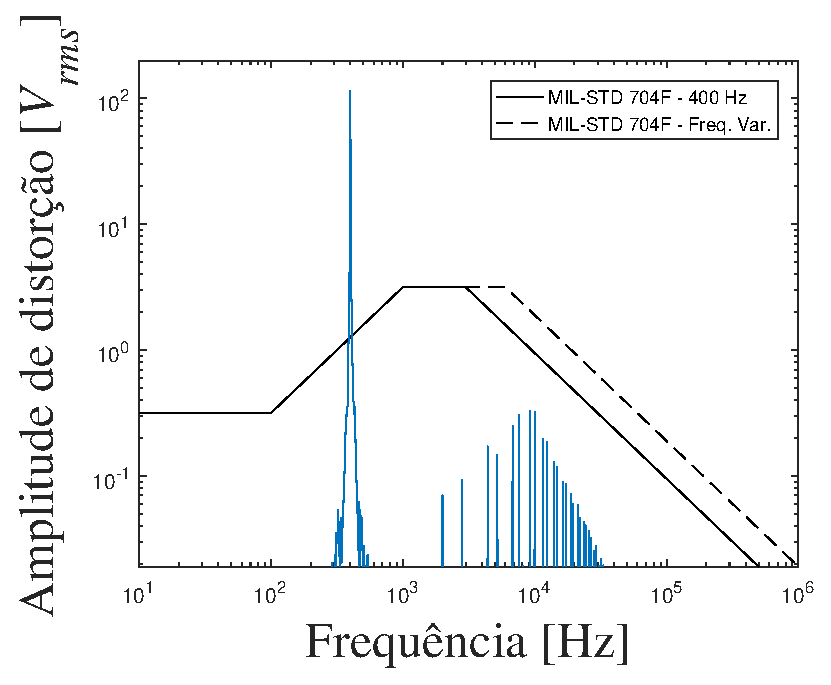
\includegraphics[width=\textwidth]{Cap4/Figuras/resultados_filt_11.eps}
		\caption{Topologia típica de um CSC}    
		\label{fig:resultados_filt_11.eps}
	\end{subfigure}%
	\caption{11}
	\label{fig:11}
\end{figure*}

\begin{figure*}[!htb] %Circuito típico de um retificador de 12 pulsos com sua respectiva corrente de entrada
	\centering
	\begin{subfigure}[b]{0.48\textwidth}
		\centering
		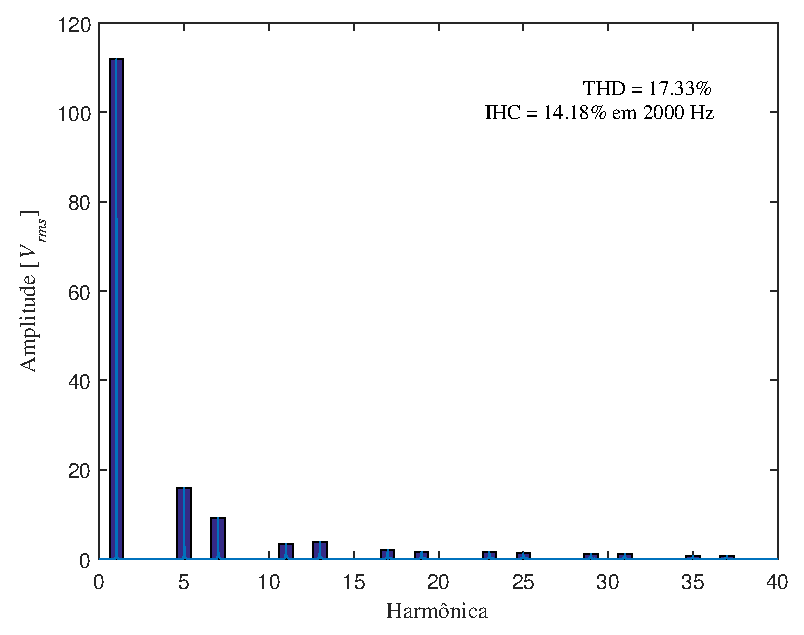
\includegraphics[width=\textwidth]{Cap4/Figuras/resultados_unfilt_12.eps}
		\caption{Topologia típica de um VSC} 
		\label{fig:resultados_unfilt_12.eps}
	\end{subfigure}%
		\hfill
	\begin{subfigure}[b]{0.48\textwidth}  
		\centering 
		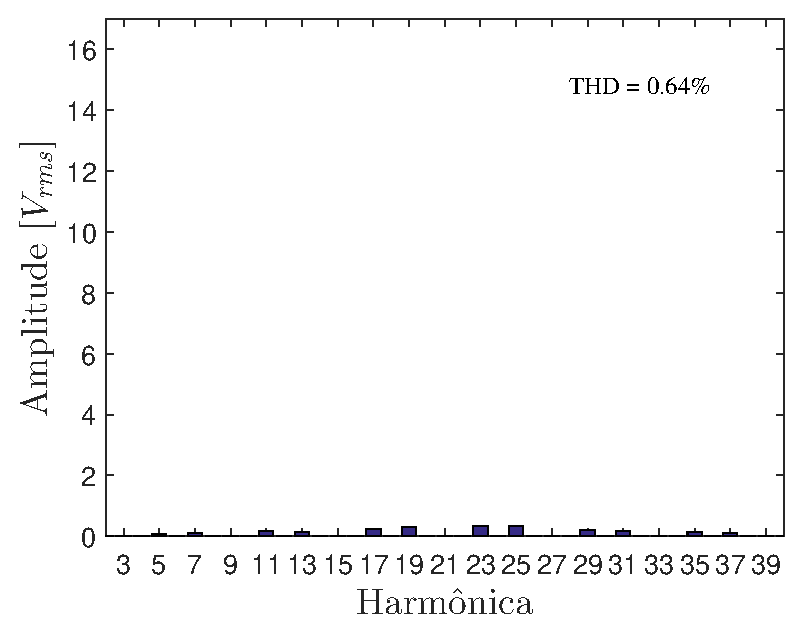
\includegraphics[width=\textwidth]{Cap4/Figuras/resultados_filt_12.eps}
		\caption{Topologia típica de um CSC}    
		\label{fig:resultados_filt_12.eps}
	\end{subfigure}%
	\caption{12}
	\label{fig:12}
\end{figure*}

\FloatBarrier

\subsubsection{Regime Transitório}

O regime transitório é mostrado na Figura \ref{fig:13} e é caracterizado pela variação da corrente no tempo sem que haja grande oscilação, como apresentado no período anterior. Esse intervalo de tempo é delimitado entre 73,3 e 73,7 segundos.

A Figura \ref{fig:14} apresenta um pequeno intervalo a qual é definido o período em que a corrente mostra-se mais elevada. Na Figura \ref{fig:resultados_unfilt_14.eps} pode ser observado que a corrente é distorcida, porém não influi significativamente na qualidade de energia, visto que a tensão apresenta-se pouco distorcida. A Figura \ref{fig:resultados_filt_14.eps} apresenta a corrente em fase e próximo de uma senoide, mostrando que o filtro opera de maneira condizente com esperado. 

Outro fator que demonstra o desempenho do filtro é a análise das potências instantâneas. As figuras \ref{fig:15} e \ref{fig:16} evidencia uma certa anulação das potência reativa e da potência oscilante ativa. Porém deve ser observado que os efeitos da comutação dos semicondutores inserem ruídos na corrente e, consequentemente, nas potências instantâneas. Outro fator a ser esclarecido nessas figuras é o fato de que o capacitor entrega certa potência no início do período estudado, de forma que a potência extraída da fonte no caso sem filtro é mais elevada que no caso com o filtro.

A análise do espectro de frequência das tensões mostra que a qualidade de energia é melhorada com a aplicação do filtro, entretanto, devido aos níveis de corrente apresentados nesse período, a operação sem filtro não apresenta distorção suficiente que descumpre a norma aeronáutica de referência.

\begin{figure*}[!htb] %Circuito típico de um retificador de 12 pulsos com sua respectiva corrente de entrada
	\centering
	\begin{subfigure}[b]{0.48\textwidth}
		\centering
		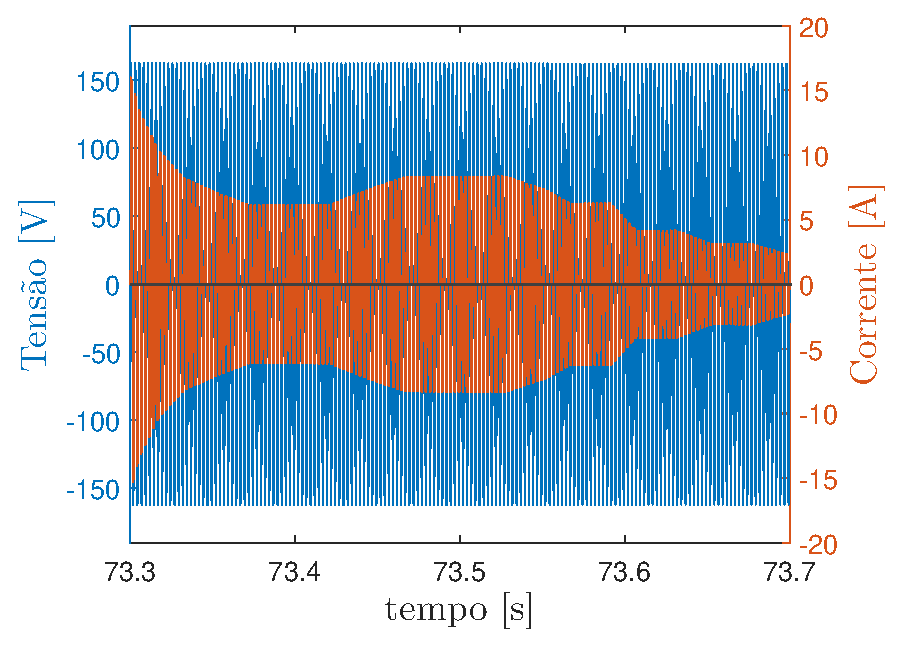
\includegraphics[width=\textwidth]{Cap4/Figuras/resultados_unfilt_13.eps}
		\caption{Topologia típica de um VSC} 
		\label{fig:resultados_unfilt_13.eps}
	\end{subfigure}%
		\hfill
	\begin{subfigure}[b]{0.48\textwidth}  
		\centering 
		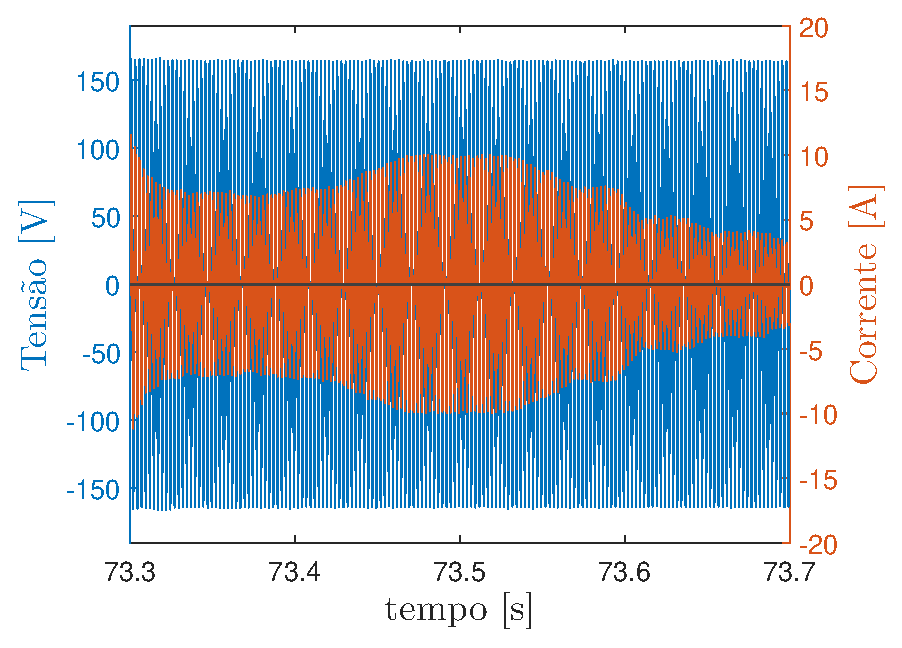
\includegraphics[width=\textwidth]{Cap4/Figuras/resultados_filt_13.eps}
		\caption{Topologia típica de um CSC}    
		\label{fig:resultados_filt_13.eps}
	\end{subfigure}%
	\caption{13}
	\label{fig:13}
\end{figure*}

\begin{figure*}[!htb] %Circuito típico de um retificador de 12 pulsos com sua respectiva corrente de entrada
	\centering
	\begin{subfigure}[b]{0.48\textwidth}
		\centering
		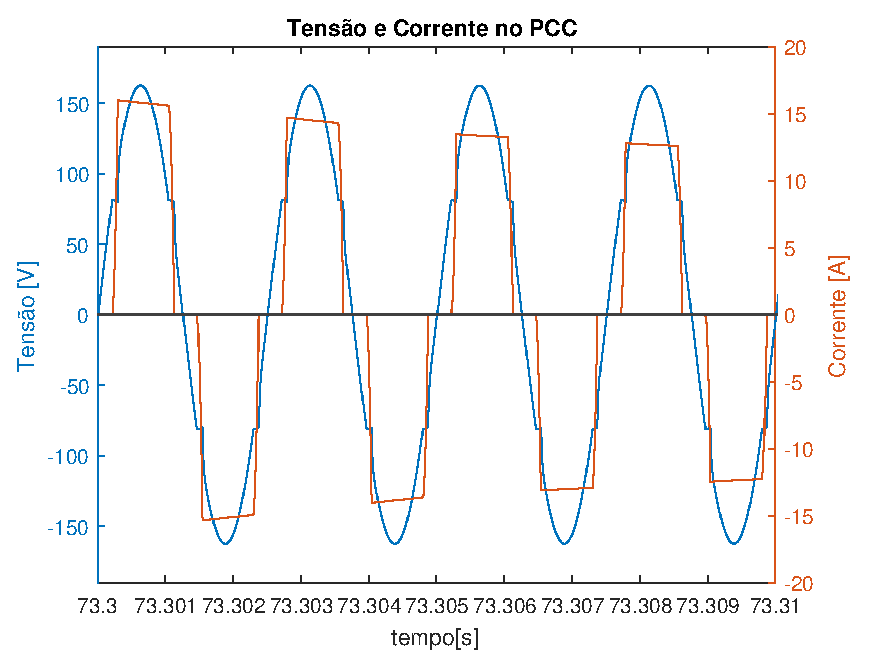
\includegraphics[width=\textwidth]{Cap4/Figuras/resultados_unfilt_14.eps}
		\caption{Topologia típica de um VSC} 
		\label{fig:resultados_unfilt_14.eps}
	\end{subfigure}%
		\hfill
	\begin{subfigure}[b]{0.48\textwidth}  
		\centering 
		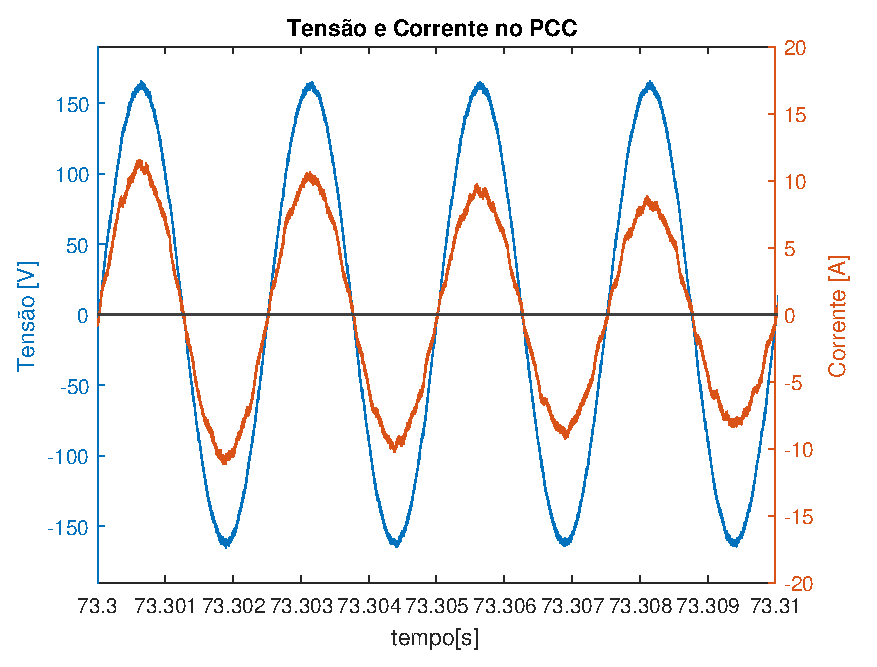
\includegraphics[width=\textwidth]{Cap4/Figuras/resultados_filt_14.eps}
		\caption{Topologia típica de um CSC}    
		\label{fig:resultados_filt_14.eps}
	\end{subfigure}%
	\caption{14}
	\label{fig:14}
\end{figure*}

\begin{figure*}[!htb] %Circuito típico de um retificador de 12 pulsos com sua respectiva corrente de entrada
	\centering
	\begin{subfigure}[b]{0.48\textwidth}
		\centering
		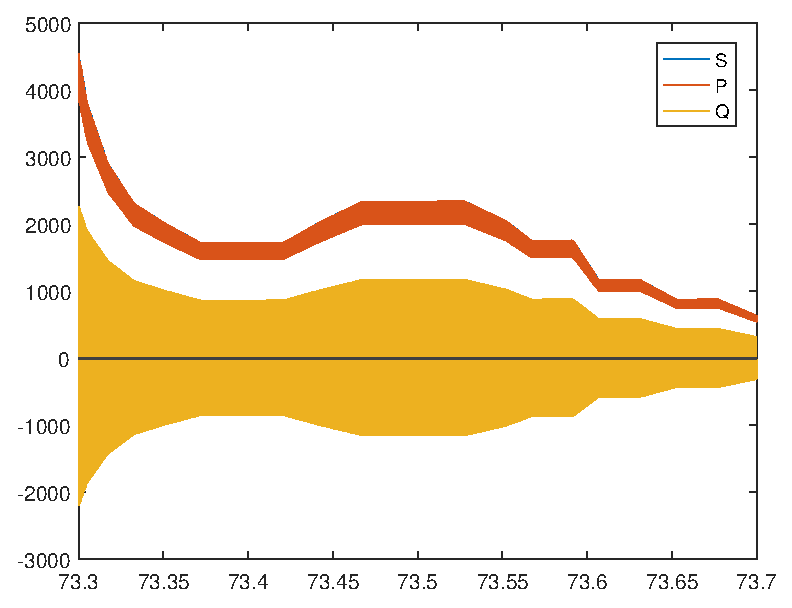
\includegraphics[width=\textwidth]{Cap4/Figuras/resultados_unfilt_15.eps}
		\caption{Topologia típica de um VSC} 
		\label{fig:resultados_unfilt_15.eps}
	\end{subfigure}%
		\hfill
	\begin{subfigure}[b]{0.48\textwidth}  
		\centering 
		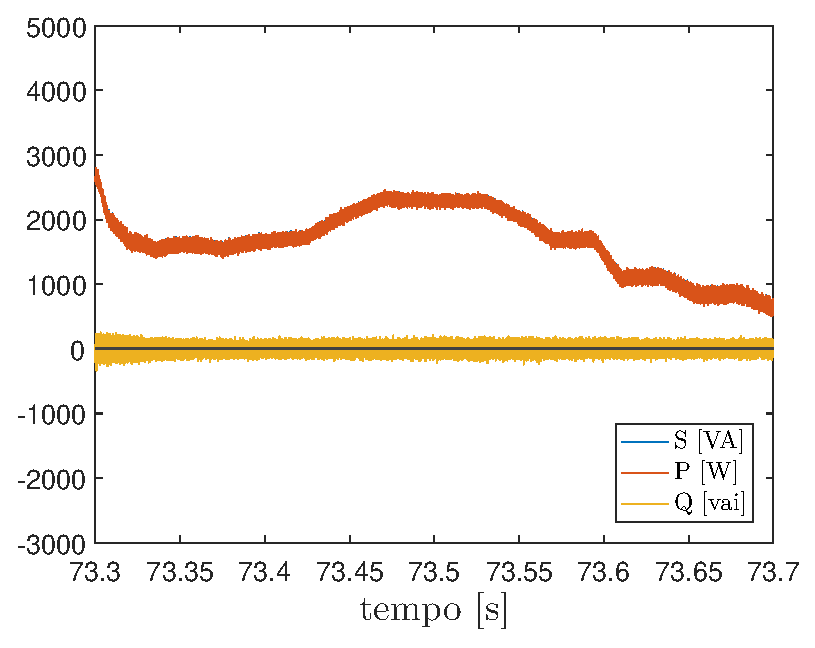
\includegraphics[width=\textwidth]{Cap4/Figuras/resultados_filt_15.eps}
		\caption{Topologia típica de um CSC}    
		\label{fig:resultados_filt_15.eps}
	\end{subfigure}%
	\caption{15}
	\label{fig:15}
\end{figure*}

\begin{figure*}[!htb] %Circuito típico de um retificador de 12 pulsos com sua respectiva corrente de entrada
	\centering
	\begin{subfigure}[b]{0.48\textwidth}
		\centering
		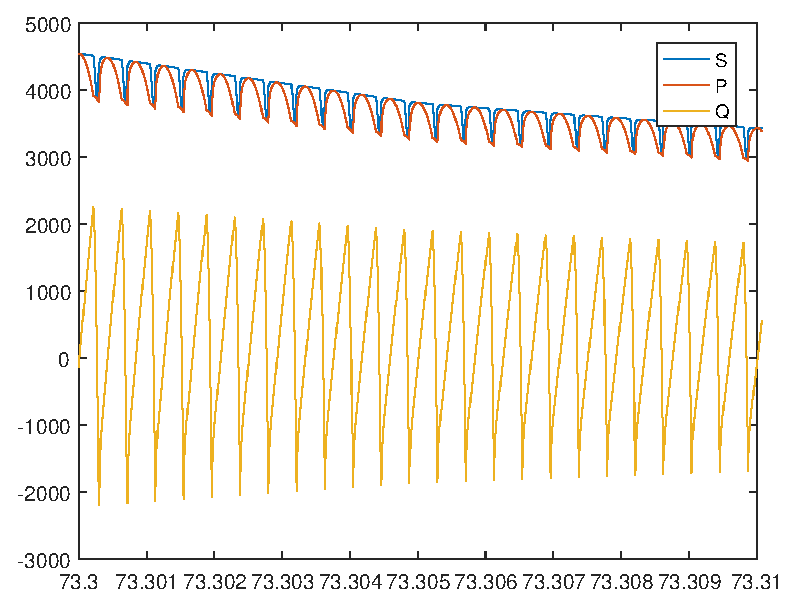
\includegraphics[width=\textwidth]{Cap4/Figuras/resultados_unfilt_16.eps}
		\caption{Topologia típica de um VSC} 
		\label{fig:resultados_unfilt_16.eps}
	\end{subfigure}%
		\hfill
	\begin{subfigure}[b]{0.48\textwidth}  
		\centering 
		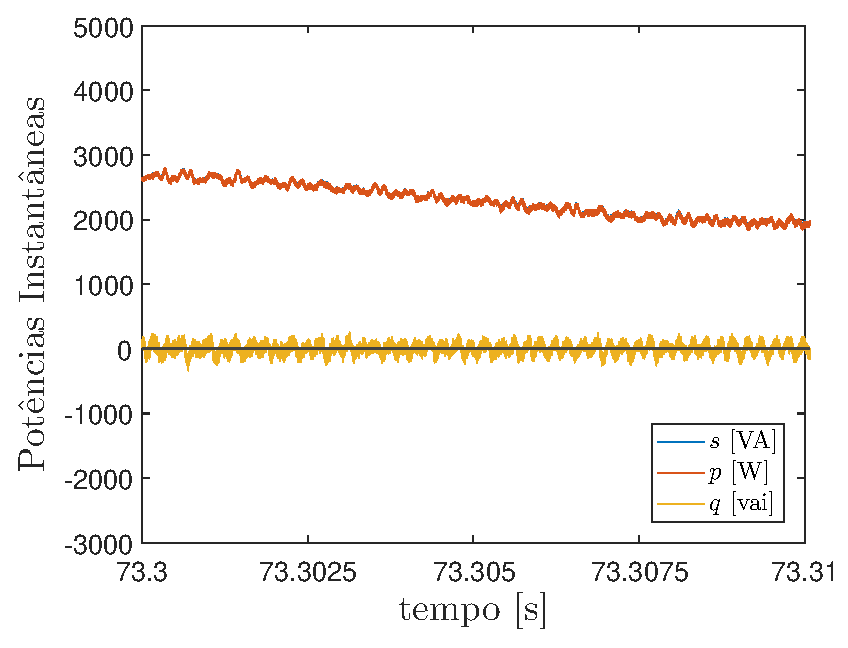
\includegraphics[width=\textwidth]{Cap4/Figuras/resultados_filt_16.eps}
		\caption{Topologia típica de um CSC}    
		\label{fig:resultados_filt_16.eps}
	\end{subfigure}%
	\caption{16}
	\label{fig:16}
\end{figure*}

\begin{figure*}[!htb] %Circuito típico de um retificador de 12 pulsos com sua respectiva corrente de entrada
	\centering
	\begin{subfigure}[b]{0.48\textwidth}
		\centering
		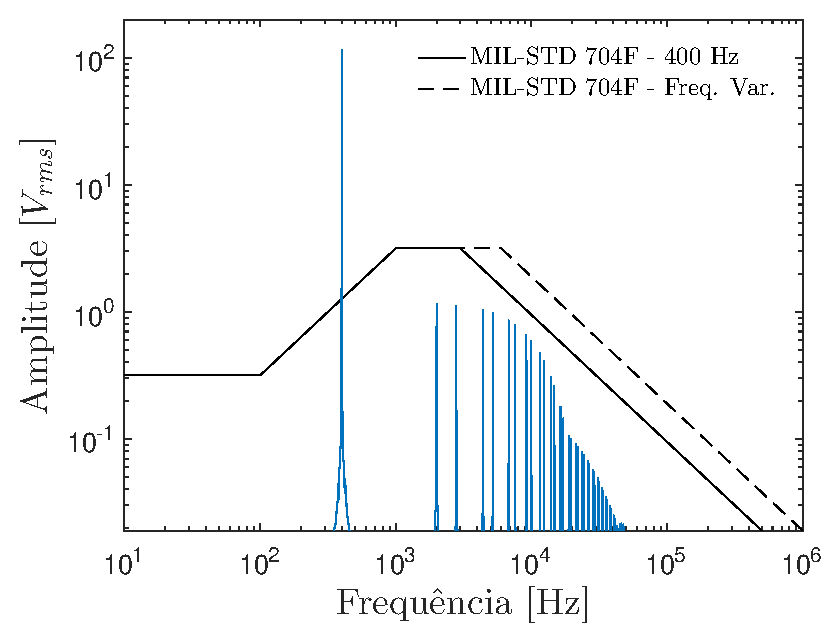
\includegraphics[width=\textwidth]{Cap4/Figuras/resultados_unfilt_17.eps}
		\caption{Topologia típica de um VSC} 
		\label{fig:resultados_unfilt_17.eps}
	\end{subfigure}%
		\hfill
	\begin{subfigure}[b]{0.48\textwidth}  
		\centering 
		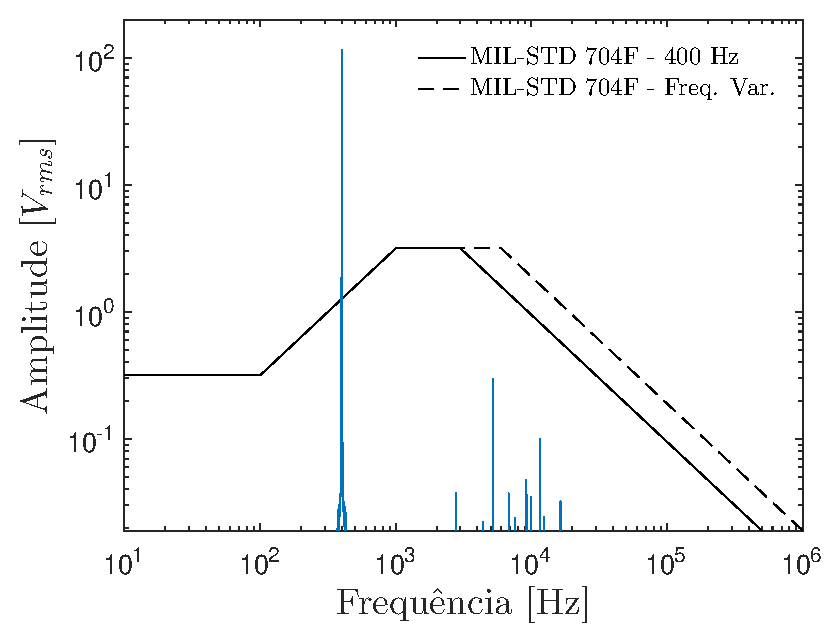
\includegraphics[width=\textwidth]{Cap4/Figuras/resultados_filt_17.eps}
		\caption{Topologia típica de um CSC}    
		\label{fig:resultados_filt_17.eps}
	\end{subfigure}%
	\caption{17}
	\label{fig:17}
\end{figure*}

\begin{figure*}[!htb] %Circuito típico de um retificador de 12 pulsos com sua respectiva corrente de entrada
	\centering
	\begin{subfigure}[b]{0.48\textwidth}
		\centering
		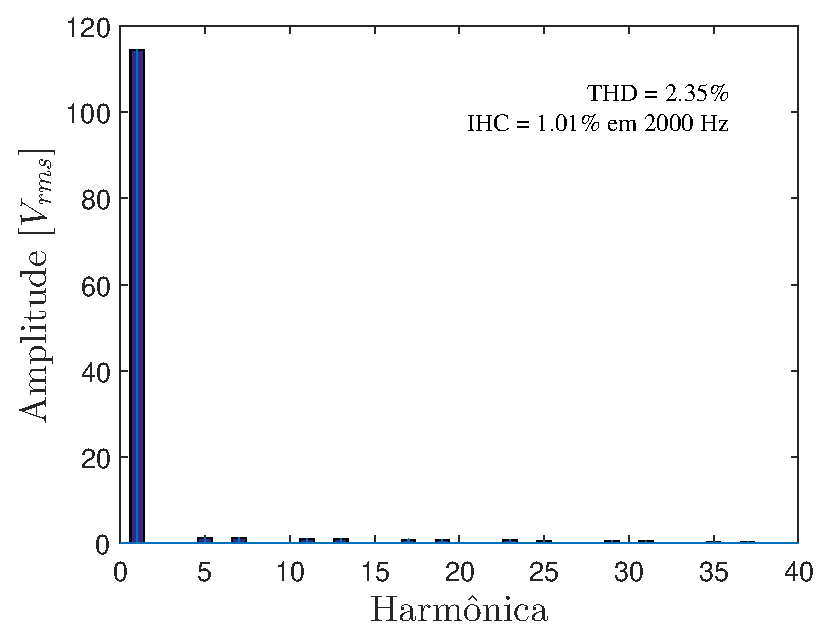
\includegraphics[width=\textwidth]{Cap4/Figuras/resultados_unfilt_18.eps}
		\caption{Topologia típica de um VSC} 
		\label{fig:resultados_unfilt_18.eps}
	\end{subfigure}%
		\hfill
	\begin{subfigure}[b]{0.48\textwidth}  
		\centering 
		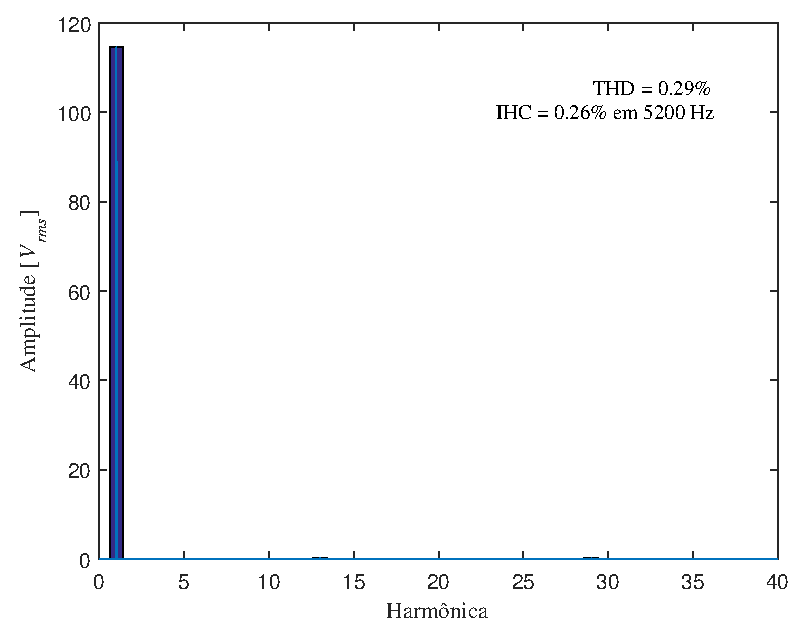
\includegraphics[width=\textwidth]{Cap4/Figuras/resultados_filt_18.eps}
		\caption{Topologia típica de um CSC}    
		\label{fig:resultados_filt_18.eps}
	\end{subfigure}%
	\caption{18}
	\label{fig:18}
\end{figure*}

\FloatBarrier

\subsubsection{Regime Permanente}

\begin{figure*}[!htb] %Circuito típico de um retificador de 12 pulsos com sua respectiva corrente de entrada
	\centering
	\begin{subfigure}[b]{0.48\textwidth}
		\centering
		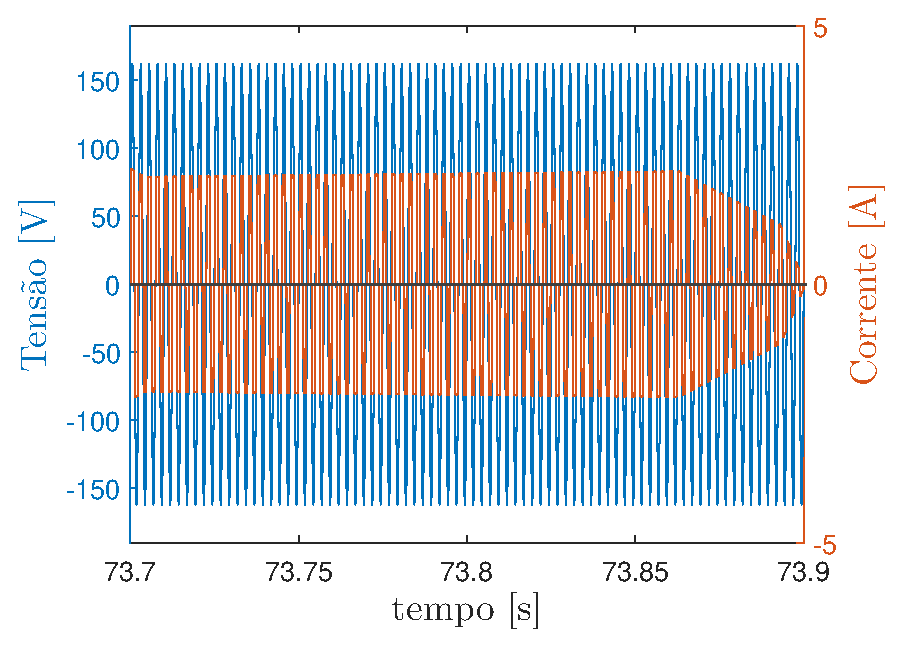
\includegraphics[width=\textwidth]{Cap4/Figuras/resultados_unfilt_19.eps}
		\caption{Topologia típica de um VSC} 
		\label{fig:resultados_unfilt_19.eps}
	\end{subfigure}%
		\hfill
	\begin{subfigure}[b]{0.48\textwidth}  
		\centering 
		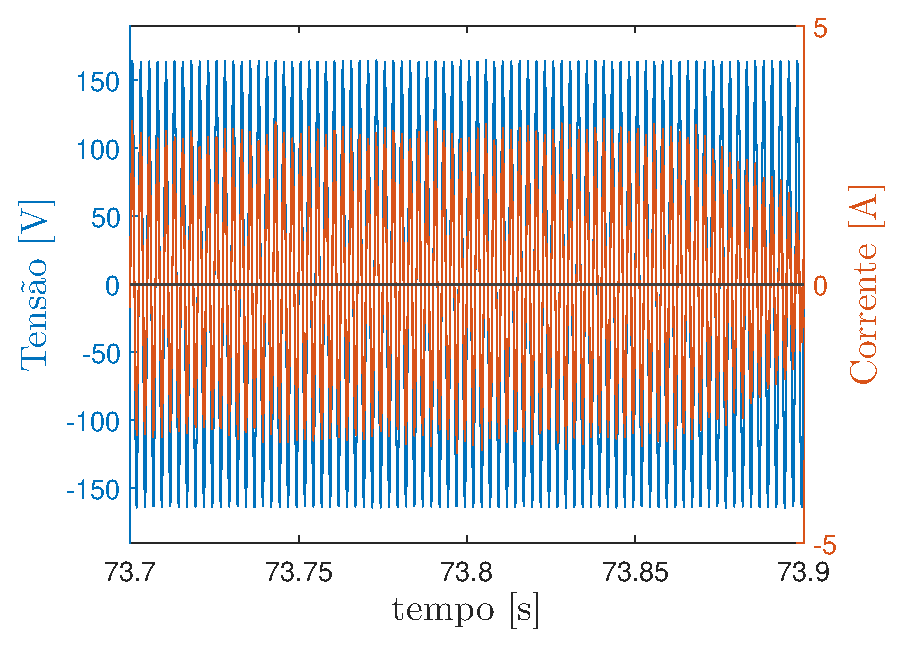
\includegraphics[width=\textwidth]{Cap4/Figuras/resultados_filt_19.eps}
		\caption{Topologia típica de um CSC}    
		\label{fig:resultados_filt_19.eps}
	\end{subfigure}%
	\caption{19}
	\label{fig:19}
\end{figure*}

\begin{figure*}[!htb] %Circuito típico de um retificador de 12 pulsos com sua respectiva corrente de entrada
	\centering
	\begin{subfigure}[b]{0.48\textwidth}
		\centering
		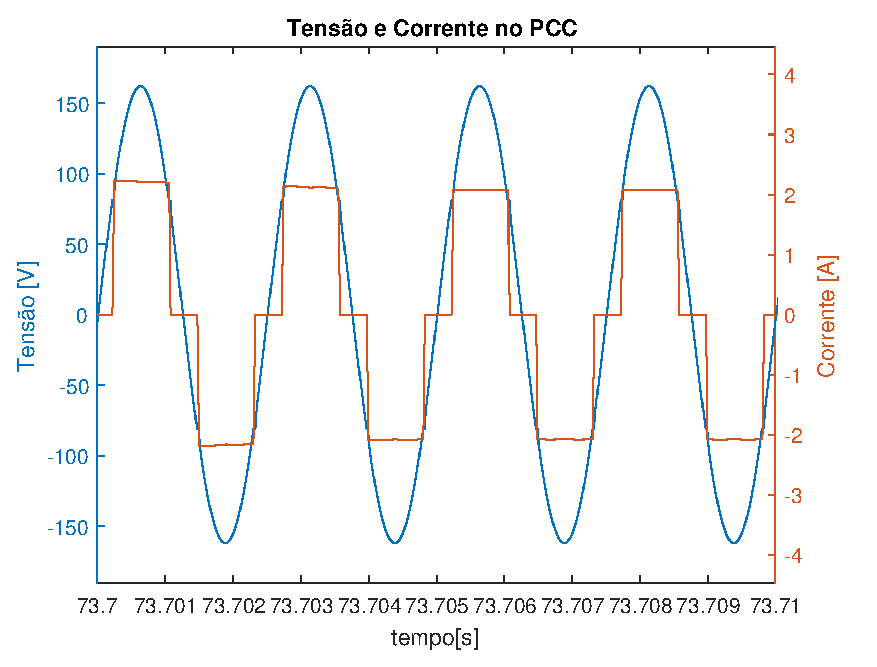
\includegraphics[width=\textwidth]{Cap4/Figuras/resultados_unfilt_20.eps}
		\caption{Topologia típica de um VSC} 
		\label{fig:resultados_unfilt_20.eps}
	\end{subfigure}%
		\hfill
	\begin{subfigure}[b]{0.48\textwidth}  
		\centering 
		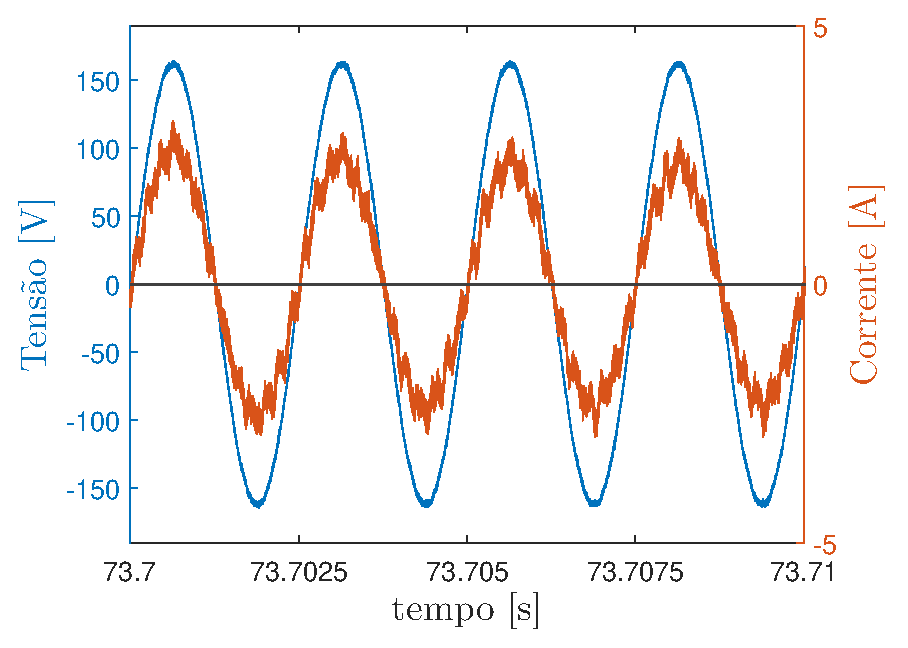
\includegraphics[width=\textwidth]{Cap4/Figuras/resultados_filt_20.eps}
		\caption{Topologia típica de um CSC}    
		\label{fig:resultados_filt_20.eps}
	\end{subfigure}%
	\caption{20}
	\label{fig:20}
\end{figure*}

\begin{figure*}[!htb] %Circuito típico de um retificador de 12 pulsos com sua respectiva corrente de entrada
	\centering
	\begin{subfigure}[b]{0.48\textwidth}
		\centering
		\includegraphics[width=\textwidth]{Cap4/Figuras/resultados_unfilt_21.eps}
		\caption{Topologia típica de um VSC} 
		\label{fig:resultados_unfilt_21.eps}
	\end{subfigure}%
		\hfill
	\begin{subfigure}[b]{0.48\textwidth}  
		\centering 
		\includegraphics[width=\textwidth]{Cap4/Figuras/resultados_filt_21.eps}
		\caption{Topologia típica de um CSC}    
		\label{fig:resultados_filt_21.eps}
	\end{subfigure}%
	\caption{21}
	\label{fig:21}
\end{figure*}

\begin{figure*}[!htb] %Circuito típico de um retificador de 12 pulsos com sua respectiva corrente de entrada
	\centering
	\begin{subfigure}[b]{0.48\textwidth}
		\centering
		\includegraphics[width=\textwidth]{Cap4/Figuras/resultados_unfilt_22.eps}
		\caption{Topologia típica de um VSC} 
		\label{fig:resultados_unfilt_22.eps}
	\end{subfigure}%
		\hfill
	\begin{subfigure}[b]{0.48\textwidth}  
		\centering 
		\includegraphics[width=\textwidth]{Cap4/Figuras/resultados_filt_22.eps}
		\caption{Topologia típica de um CSC}    
		\label{fig:resultados_filt_22.eps}
	\end{subfigure}%
	\caption{22}
	\label{fig:22}
\end{figure*}

\begin{figure*}[!htb] %Circuito típico de um retificador de 12 pulsos com sua respectiva corrente de entrada
	\centering
	\begin{subfigure}[b]{0.48\textwidth}
		\centering
		\includegraphics[width=\textwidth]{Cap4/Figuras/resultados_unfilt_23.eps}
		\caption{Topologia típica de um VSC} 
		\label{fig:resultados_unfilt_23.eps}
	\end{subfigure}%
		\hfill
	\begin{subfigure}[b]{0.48\textwidth}  
		\centering 
		\includegraphics[width=\textwidth]{Cap4/Figuras/resultados_filt_23.eps}
		\caption{Topologia típica de um CSC}    
		\label{fig:resultados_filt_23.eps}
	\end{subfigure}%
	\caption{23}
	\label{fig:23}
\end{figure*}

\begin{figure*}[!htb] %Circuito típico de um retificador de 12 pulsos com sua respectiva corrente de entrada
	\centering
	\begin{subfigure}[b]{0.48\textwidth}
		\centering
		\includegraphics[width=\textwidth]{Cap4/Figuras/resultados_unfilt_24.eps}
		\caption{Topologia típica de um VSC} 
		\label{fig:resultados_unfilt_24.eps}
	\end{subfigure}%
		\hfill
	\begin{subfigure}[b]{0.48\textwidth}  
		\centering 
		\includegraphics[width=\textwidth]{Cap4/Figuras/resultados_filt_24.eps}
		\caption{Topologia típica de um CSC}    
		\label{fig:resultados_filt_24.eps}
	\end{subfigure}%
	\caption{24}
	\label{fig:24}
\end{figure*}

\FloatBarrier
